\section{DeepCut Results}
\label{sec:experiments:multicut}
The aim of this paper is to tackle the multi person case. To that end,
we evaluate the proposed $\deepcut$ models on four diverse
benchmarks. We confirm that both single person ($\singb$) and
multi person ($\multb$) variants (Sec.~\ref{section:problem}) are
effective on standard $\singb$ pose estimation
datasets~\cite{johnson10bmvc,andriluka14cvpr}.
%% described in
%%Sec.~\ref{section:unary}.
%Both types of models
%perform equally well, slightly improving over unaries only and
%significantly outperforming state of the art.
Then, we demonstrate superior performance of $\deepcut~\multb$ on the
multi person pose estimation task.

\begin{figure}
  \centering
  \begin{tabular}{c c}  
  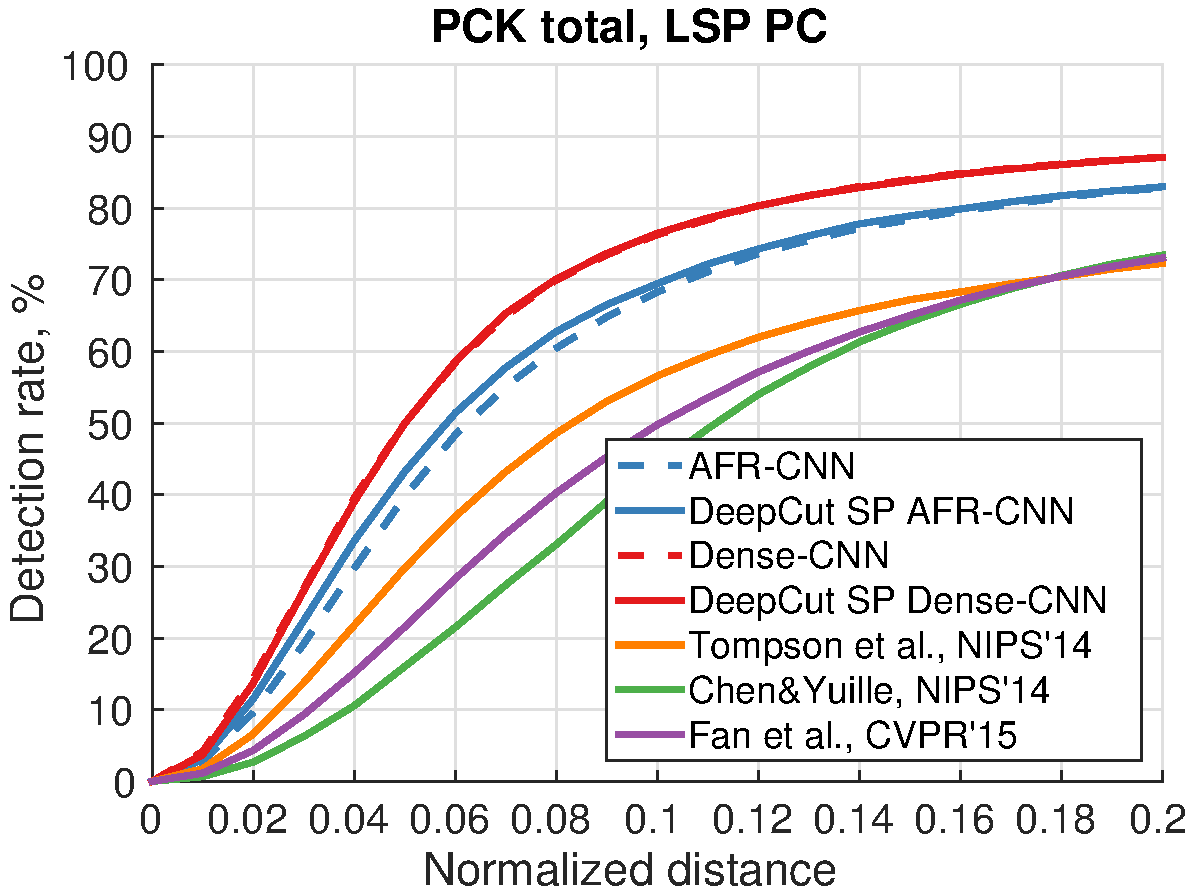
\includegraphics[width=0.48\linewidth]{pck-total-lsp-PC.pdf}&
  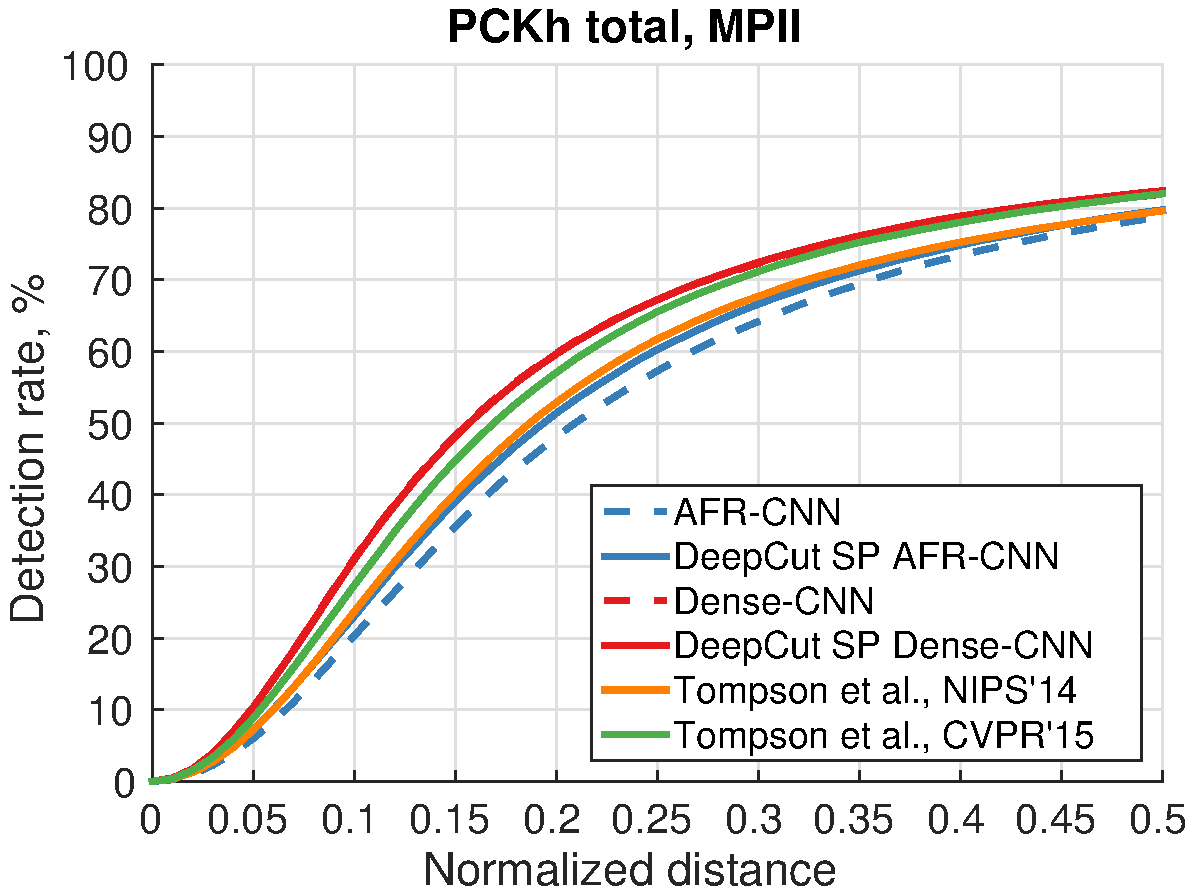
\includegraphics[width=0.48\linewidth]{pckh-total-mpii.pdf}\\
  (a) LSP (PC)& (b) MPII Single Person \\
  \end{tabular}
  \vspace{-0.1em}
%  \caption{Pose estimation performance on (a) LSP (PC) dataset (PCK) and (b) MPII Single Person dataset (PCKh).} 
  \caption{Pose estimation results over all PCK thresholds.} 
    \vspace{-1.2em}
  \label{fig:pck-curves}
\end{figure}


\subsection{Single Person Pose Estimation}
\label{sec:multicut:single}
We now evaluate single person (\textit{SP}) and more general
multi person (\textit{MP}) $\deepcut$ models on LSP and MPII $\singb$
benchmarks described in Sec.~\ref{section:unary}. Since this
evaluation setting implicitly relies on the knowledge that all parts
are present in the image we always output the full number of parts.
% BERNT: I would not include the following sentence as such
% if you want to totally clear we should rephrase this as to make this
% more compelling
%To that end we use
%hypothesis with the highest unary score when the body part predicted
%as occluded.
%\renewcommand{\tabcolsep}{0.15cm}
\tabcolsep 1.5pt
\begin{table}[tbp]
 \scriptsize
  \centering
  \begin{tabular}{@{} l c ccc ccc c|c@{}}
    \toprule
    Setting& Head   & Sho  & Elb & Wri & Hip & Knee & Ank & PCK & AUC\\       
    \midrule
    $\rcnn$ (unary) & 95.4  & 86.5  & 77.8  & 74.0  & 84.5  & 82.6 & 78.8 & 82.8 & 57.0\\



    \quad+ $\deepcut$ \singb& 95.4  & 86.7  & 78.3  & 74.0  & 84.3  & 82.9 & 79.2& 83.0 & 58.4 \\


    \quad\quad+ appearance pairwise & 95.4  & 87.2  & 78.6  & 73.7  & 84.7  & 82.8 & 78.8 & 83.0 & 58.5 \\

    \quad+ $\deepcut$ \multb & 95.2  & 86.7  & 78.2  & 73.5  & 84.6  & 82.8 & 79.0 & 82.9 & 58.0\\

 
    \midrule
    $\dense$ (unary)                   & \textbf{97.2}  & 90.8  & 83.0  & \textbf{79.3}  & 90.6  & 85.6 & \textbf{83.1} & \textbf{87.1} & \textbf{63.6}\\
    %\quad + $\deepcuts~\singb$ & 97.0  & \textbf{91.1}  & \textbf{83.9}  & 77.8  & 90.7  & \textbf{86.7} & 81.0 & 86.9 & 63.4\\
    \quad + $\deepcut~\singb$ & 97.0  & 91.0  & \textbf{83.8}  & 78.1  & 91.0  & 86.7 & 82.0 & \textbf{87.1} & 63.5\\
    \quad + $\deepcut~\multb$& 96.2  & \textbf{91.2}  & 83.3  & 77.6  & \textbf{91.3}  & \textbf{87.0} & 80.4 & 86.7 & 62.6 \\

 
    \midrule
    %Tompson et al.~\cite{tompson14nips} (unary)  & 88.3 & 77.3 & 66.1 & 62.7 & 66.6 & 68.3 & 65.0 & 70.6 \\
    Tompson et al.~\cite{tompson14nips}& 90.6  & 79.2  & 67.9  & 63.4  & 69.5  & 71.0 & 64.2 & 72.3 & 47.3\\
    Chen\&Yuille~\cite{chen14nips}& 91.8  & 78.2  & 71.8  & 65.5  & 73.3  & 70.2 & 63.4& 73.4 & 40.1\\
    Fan et al.~\cite{fan15cvpr}$^*$
    & 92.4 & 75.2& 65.3& 64.0& 75.7& 68.3& 70.4& 73.0 & 43.2 \\
    \bottomrule
  \end{tabular}
  
  $^*$ re-evaluated using the standard protocol, for details see project page of \cite{fan15cvpr}
  \caption[]{Pose estimation results (PCK) on LSP (PC) dataset.}
    \vspace{-1.5em}
  \label{tab:multicut:lsp}
\end{table}


\myparagraph{Results on LSP.} We report per-part PCK results
(Tab.~\ref{tab:multicut:lsp}) and results for a variable distance
threshold (Fig.~\ref{fig:pck-curves} (a)). $\deepcut~\singb~\rcnn$
model using $100$ detections improves over unary only ($83.0$
vs. $82.8$\%~PCK, $58.4$ vs. $57$\% AUC), as pairwise connections
filter out some of the high-scoring detections on the background. The
improvement is clear in Fig.~\ref{fig:pck-curves}~(a) for smaller
thresholds. Using part appearance scores in addition to geometrical
features in $c\neq c'$ pairwise terms only slightly improves AUC, as
the appearance of neighboring parts is mostly captured by a relatively
large region centered at each part. 
%% As geometrical only pairwise lead
%% to faster convergence, we use them in the rest of the
%% experiments. 
The performance of $\deepcut~\multb~\rcnn$ matches the
$\singb$ and improves over $\rcnn$ alone: $\deepcut~\multb$ correctly
handles the $\singb$ case. Performance of $\deepcut~\singb~\dense$ is
almost identical to unary only, unlike the results for
$\rcnn$. $\dense$ performance is noticeably higher compared to
$\rcnn$, and ``easy'' cases that could have been corrected by a
spatial model are resolved by stronger part detectors alone.

\myparagraph{Comparison to the state of the art (LSP).}
Tab.~\ref{tab:multicut:lsp} compares results of $\deepcut$ models to
other deep learning methods specifically designed for single person
pose estimation. All $\deepcuts$ significantly outperform the state of
the art, with $\deepcut~\singb~\dense$ model improving by $13.7$\% PCK
over the best known result~\cite{chen14nips}. The improvement is even
more dramatic for lower thresholds (Fig.~\ref{fig:pck-curves}~(a)):
for PCK @ $0.1$ the best model improves by $19.9$\% over Tompson et
al.~\cite{tompson14nips}, by $26.7$\% over Fan et al.~\cite{fan15cvpr},
and by $32.4$\%~PCK over Chen\&Yuille~\cite{chen14nips}. The latter is
interesting, as~\cite{chen14nips} use a stronger spatial model that
predicts the pairwise conditioned on the CNN features, whereas
$\deepcuts$ use geometric-only pairwise connectivity. Including body
part orientation information into $\deepcuts$ should further improve
the results.

\myparagraph{Results on MPII Single Person.} Results are shown in
Tab.~\ref{tab:multicut:mpii} and Fig.~\ref{fig:pck-curves}
(b). $\deepcut~\singb~\rcnn$ noticeably improves over $\rcnn$ alone
($79.8$ vs. $78.8$\%~PCK, $51.1$ vs. $49.0$\% AUC). The improvement is
stronger for smaller thresholds (c.f. Fig.~\ref{fig:pck-curves}), as
spatial model improves part localization. $\dense$ alone trained on
MPII outperforms $\rcnn$ ($81.6$ vs. $78.8$\% PCK), which shows the
advantages of dense training and evaluation. As expected, $\dense$
performs slightly better when trained on the larger
MPII+LSPET. Finally, $\deepcut~\dense~\singb$ is slightly better than
$\dense$ alone leading to the best result on MPII dataset ($82.4$\%
PCK).

\myparagraph{Comparison to the state of the art (MPII).} We compare
the performance of $\deepcut$ models to the best deep learning
approaches from the
literature~\cite{tompson14nips,Tompson:2015:EOL}\footnote{\cite{tompson14nips}
  was re-trained and evaluated on MPII dataset by the
  authors.}.
%% \cite{tompson14nips} is a fully-convolutional deep architecture
%% relying on multi-resolution filter banks that have various receptive
%% field sizes. In addition, this model jointly trains part detectors and
%% spatial model in the same deep architecture. This model was kindly
%% re-trained by the authors on the MPII dataset for fair
%% comparison. \cite{Tompson:2015:EOL} is an extension of
%% \cite{tompson14nips} and it specifically trains a separate deep
%% full-convolutional model for location refinement. The results are
%% shown in Tab.~\ref{tab:multicut:mpii}.
$\deepcut~\singb~\dense$ outperforms
both~\cite{tompson14nips,Tompson:2015:EOL} ($82.4$ vs $79.6$ and $82.0$\%
PCK, respectively). Similar to them $\deepcuts$ rely on dense training
and evaluation of part detectors, but unlike them use single size
receptive field and do not include multi-resolution context
information. Also, appearance and spatial components of $\deepcuts$
are trained piece-wise, unlike~\cite{tompson14nips}. We observe that
performance differences are higher for smaller thresholds
(c.f. Fig.~\ref{fig:pck-curves}~(b)). This is remarkable, as a much
simpler strategy for location refinement is used compared
to~\cite{Tompson:2015:EOL}. Using multi-resolution filters and joint
training should improve the performance.
%% We believe that training a separate deep
%% convolutional model for location refinement should further improve
%% results.

%\renewcommand{\tabcolsep}{0.15cm}
\tabcolsep 1.5pt
\begin{table}[tbp]
 \scriptsize
  \centering
  \begin{tabular}{@{} l c ccc ccc c|c@{}}
    \toprule
    Setting& Head   & Sho  & Elb & Wri & Hip & Knee & Ank & PCK$_h$ & AUC\\
    \midrule
    %Fast R-CNN MPII& 91.5  & 89.8  & 80.6  & 74.2  & 76.7  & 69.4 & 63.0 & 81.6 & 78.7 & 48.7 \\
%Fast R-CNN MPII& 91.5  & 89.8  & 80.6  & 74.2  & 76.7  & 69.4 & 63.0 & 78.7 & 48.7 \\
$\rcnn$ (unary) & 91.5  & 89.7  & 80.5  & 74.4  & 76.9  & 69.6 & 63.1 & 78.8 & 49.0\\

    %Fast R-CNN MPII~\singb& 92.3  & 90.8  & 81.6  & 74.9  & 79.0  & 70.2 & 63.0 & 79.7 & 50.8 \\
\quad+ $\deepcut$ \singb& 92.3  & 90.6  & 81.7  & 74.9  & 79.2  & 70.4 & 63.0 & 79.8 &51.1\\


    \midrule
    $\dense$ (unary)              & 93.5  & 88.6  & 82.2  & 77.1  & 81.7  & 74.4 & \textbf{68.9} & 81.6 & 56.0\\
    \quad+LSPET        & 94.0  & 89.4  & 82.3  & 77.5  & 82.0          & 74.4          & 68.7          & 81.9          & \textbf{56.5} \\
    \quad\quad+$\deepcut$ \singb& 94.1  & 90.2  & 83.4  & 77.3  & \textbf{82.6} & \textbf{75.7} & 68.6          & \textbf{82.4} & \textbf{56.5} \\
    \midrule
    Tompson et al.~\cite{tompson14nips}  &95.8 & 90.3 & 80.5 & 74.3 & 77.6 & 69.7 & 62.8 & 79.6 & 51.8\\
    Tompson et al.~\cite{Tompson:2015:EOL}  &\textbf{96.1} & \textbf{91.9} & \textbf{83.9} &\textbf{77.8} & 80.9 & 72.3 & 64.8 & 82.0 & 54.9\\
    \bottomrule
  \end{tabular}
  \vspace{0.1em}     
  \caption[]{Pose estimation results (PCK$_h$) on MPII Single Person.}
    \vspace{-1.5em}
  \label{tab:multicut:mpii}
\end{table}


\subsection{Multi Person Pose Estimation}
We now evaluate $\deepcut~\multb$ models on the challenging task of
$\multb$ pose estimation with an unknown number of people per image
and visible body parts per person.
%% In this
%% evaluation we use the variants $\mult$ and $\multu$ of our model since
%% they demonstrated performance comparable to more costly variants in
%% previous experiments.  \todo{I don't think "mlt" = MP60 and "mltu" =
%%   MP60,UB are mentioned before?}

\myparagraph{Datasets.} For evaluation we use two public $\multb$
benchmarks: ``We Are Family'' (WAF)~\cite{eichner10eccv} with $350$
training and $175$ testing group shots of people;
%% staying close to each other and often occluding each other, the
%% images contain six people on average;
``MPII Human Pose'' (``Multi-Person'') ~\cite{andriluka14cvpr}
consisting of $3844$ training
%% images with $9687$ people
and $1758$ testing groups
%%  with $4484$ individuals involved into hundreds of every day
%% activities.
of multiple interacting individuals in highly articulated poses with
variable number of parts. On MPII, we use a subset of $288$ testing
images for evaluation.
%% The number, location and scale of
%% individuals is unknown.
%% On average there are three people per image.
%% Sample images are shown in Fig.~\ref{fig:teaserfig}.
We first pre-finetune both $\rcnn$ and $\dense$ from ImageNet to MPII
and MPII+LSPET, respectively, and further finetune each model to WAF
and MPII Multi-Person. For WAF, we re-train the spatial model on WAF
training set.
%% : it leads to better results, as poses in
%% WAF dataset are more constrained compared to MPII.

\myparagraph{WAF evaluation measure.} Approaches are evaluated using
the official toolkit~\cite{eichner10eccv}, thus results are directly
comparable to prior work. The toolkit implements occlusion-aware
``Percentage of Correct Parts ($m$PCP)'' metric. In addition, we
report ``Accuracy of Occlusion Prediction
(AOP)''~\cite{Chen:2015:POC}.

\myparagraph{MPII Multi-Person evaluation measure.} PCK metric is
suitable for $\singb$ pose estimation with known number of parts and
does not penalize for false positives that are not a part of the
ground truth.
% due to occlusion or truncation.
Thus, for $\multb$ pose estimation we use ``Mean Average Precision
(mAP)'' measure, similar to \cite{Sun:2011:APM,yang12pami}. In
contrast to~\cite{Sun:2011:APM,yang12pami} evaluating the detection of
\emph{any} part instance in the image disrespecting inconsistent pose
predictions, we evaluate consistent part configurations. First,
multiple body pose predictions are generated and then assigned to the
ground truth (GT) based on the highest
PCK$_h$~\cite{andriluka14cvpr}. Only single pose can be assigned to
GT. Unassigned predictions are counted as false positives. Finally, AP
for each body part is computed and mAP is reported.

\myparagraph{Baselines.} To assess the performance of $\rcnn$ and
$\dense$ we follow a traditional route from the literature based on
two stage approach: first a set of regions of interest (\emph{ROI}) is
generated and then the $\singb$ pose estimation is performed in the
\emph{ROIs}. This corresponds to unary only performance. \emph{ROI}
are either based on a ground truth ($\gtroi$) or on the people
detector output ($\detroi$).

%\renewcommand{\tabcolsep}{0.15cm}
\tabcolsep 1.5pt
\begin{table}[tbp]
 \scriptsize
  \centering
  \begin{tabular}{@{} l c cc cc |c@{}}
    \toprule
    Setting& Head   & U Arms  & L Arms & Torso & $m$PCP  & AOP \\
    \midrule
    \rcnn~\detroi & 69.8 & 46.0 & 36.7 & 83.7 & 53.1 & 73.9 \\

    \deepcut~\multb~\rcnn & 99.0 & 79.5 & 74.3 & 87.1 & 82.2 & 85.6 \\

    %Fast R-CNN~\multb~+ torso & 96.7 & 78.8 & 74.1 & 83.7 & 81.0 & 84.6 \\

    %Fast R-CNN~\multb~+ torso eval& 90.9 & 78.8 &  74.1 & 83.8 & 80.1 & 84.7 \\

    \midrule
    %%Dense \textit{MP100} & 96.7 & 78.9 & 80.6 & 77.3 & 78.9 & 83.7 & 82.7 & 84.7 \\
Dense \textit{MP100} & 96.7 & 79.8 & 78.1 & 83.7 & 82.7 & 84.7 \\

    %%Dense \textit{MP125} & 96.7 & 81.0 & 83.1 & 78.1 & 81.2 & 83.7 & 84.0 & 86.0 \\
Dense \textit{MP125} & 96.7 & \textbf{82.1} & \textbf{79.7} & 83.7 & \textbf{84.0} & \textbf{86.0} \\

    %Dense \multb~\etad{11/2} \\
    \dense~\detroi & 76.0 & 46.0 & 40.2 & 83.7 & 55.3 & 73.8\\

    %                               99.3 & 81.6 & 81.4 & 79.2 & 79.7 & 87.1 & 84.7 & 86.5
%Dense FaceDet \textit{MP125} & 96.7 & 81.8 & 81.6 & 78.9 & 79.7 & 83.5 & 83.7 & 85.9 \\
%Dense FaceDet \textit{MP125} & 96.7 & 81.7 & 79.3 & 83.5 & 83.7 & 85.9 \\
\deepcut~\multb~\dense & \textbf{99.3} & \textbf{81.5} & \textbf{79.5} & 87.1 & \textbf{84.7} & \textbf{86.5}\\

    %Dense \multbc~+ torso \etad{11/2} \\
    \midrule
    Ghiasi et. al.~\cite{ghiasi14cvpr}  & -      & -      & -      & -         & 63.6  &  74.0 \\
    Eichner\&Ferrari~\cite{eichner10eccv}   & 97.6   & 68.2  &   48.1     &86.1    &69.4   & 80.0 \\
    Chen\&Yuille~\cite{Chen:2015:POC}  & 98.5 &   77.2 &  71.3 &   \textbf{88.5} &   80.7 &   84.9 \\
    \bottomrule
  \end{tabular}
    \vspace{0.1em}
  \caption[]{Pose estimation results ($m$PCP) on WAF dataset.}
    \vspace{-1.0em}
  \label{tab:multicut:waf}
\end{table}


\myparagraph{Results on WAF.} Results are shown in
Tab.~\ref{tab:multicut:waf}. $\detroi$ is obtained by extending
provided upper body detection boxes.
%% by $2h$ towards the bottom of the
%% image, and then by $0.1\times h$ in all directions, where $h$ is the
%% height of the original bounding box.
$\rcnn~\detroi$ achieves $57.6$\% $m$PCP and $73.9$\%
AOP. $\deepcut~\multb~\rcnn$ significantly improves over
\rcnn~\detroi~achieving $82.2$\% $m$PCP. This improvement is stronger
compared to LSP and MPII due to several reasons. First, $m$PCP
requires consistent prediction of body sticks as opposite to body
joints, and including spatial model enforces consistency. Second,
$m$PCP metric is occlusion-aware. $\deepcuts$ can deactivate
detections for the occluded parts thus effectively reasoning about
occlusion. This is supported by strong increase in AOP ($85.6$
vs. $73.9$\%). Results by $\deepcut~\multb~\dense$ follow the same
tendency achieving the best performance of $84.7$\% $m$PCP and $86.5$\%
AOP. Both increase in $m$PCP and AOP show the advantages of
$\deepcuts$ over traditional \detroi~approaches.

Tab.~\ref{tab:multicut:waf} shows that 
%comparison to prior
%work. 
$\deepcuts$ outperform all prior methods.
%other
%methods. 
%$\deepcuts~\multb~\dense$ outperforms 
Deep learning method~\cite{Chen:2015:POC} is outperformed both for
$m$PCP (84.7 vs. 80.7\%) and AOP (86.5 vs. 84.9\%) measures. This is
remarkable, as $\deepcuts$ reason about part interactions across
several people, whereas~\cite{Chen:2015:POC} primarily focuses on the
single-person case and handles multi-person scenes akin to
\cite{yang12pami}. In contrast to~\cite{Chen:2015:POC}, $\deepcuts$
are not limited by the number of possible occlusion patterns and cover
person-person occlusions and other types as truncation and occlusion
by objects in one formulation. $\deepcuts$ significantly
outperform~\cite{eichner10eccv} while being more general:
%% who achieve good
%% performance considering much weaker part detectors based on
%% handcrafted features.
unlike~\cite{eichner10eccv} $\deepcuts$ do not require person detector
and not limited by a number of occlusion states among people.

Qualitative comparison to ~\cite{Chen:2015:POC} is provided in
Fig.~\ref{fig:qualitative_waf_2}.

\begin{figure*}
  \centering
  \begin{tabular}{c c c c c c}
  \begin{sideways}\bf \small \quad\quad $\detroi$\end{sideways}&
  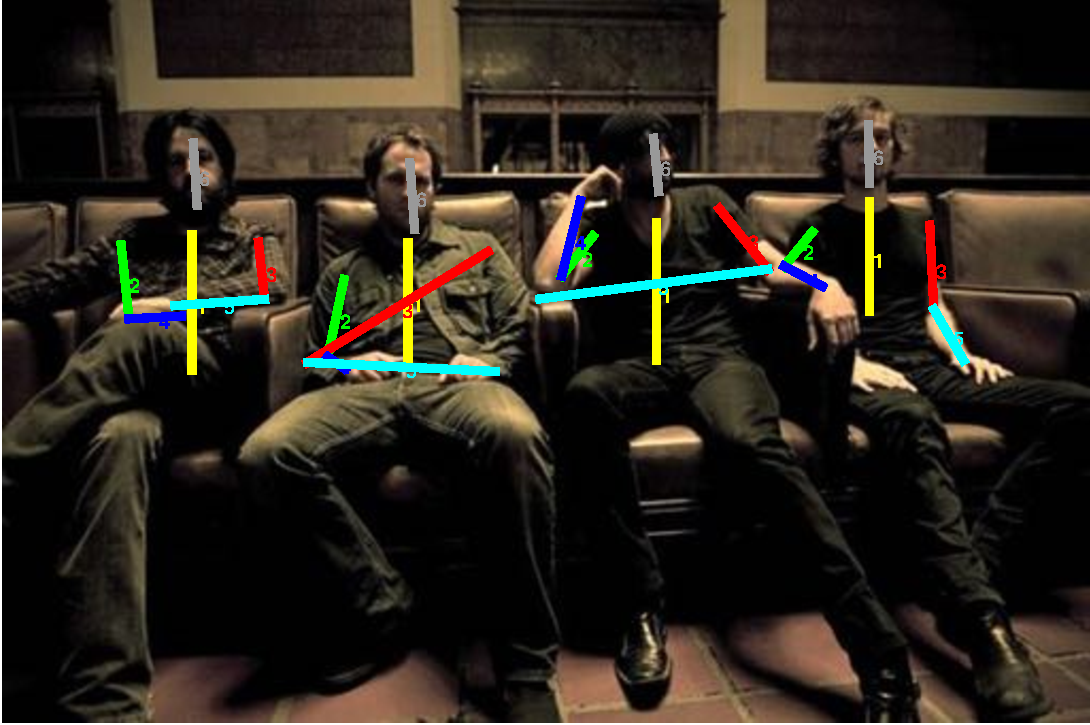
\includegraphics[height=0.150\linewidth]{imgidx_0012_sticks_unary_waf.pdf}&
  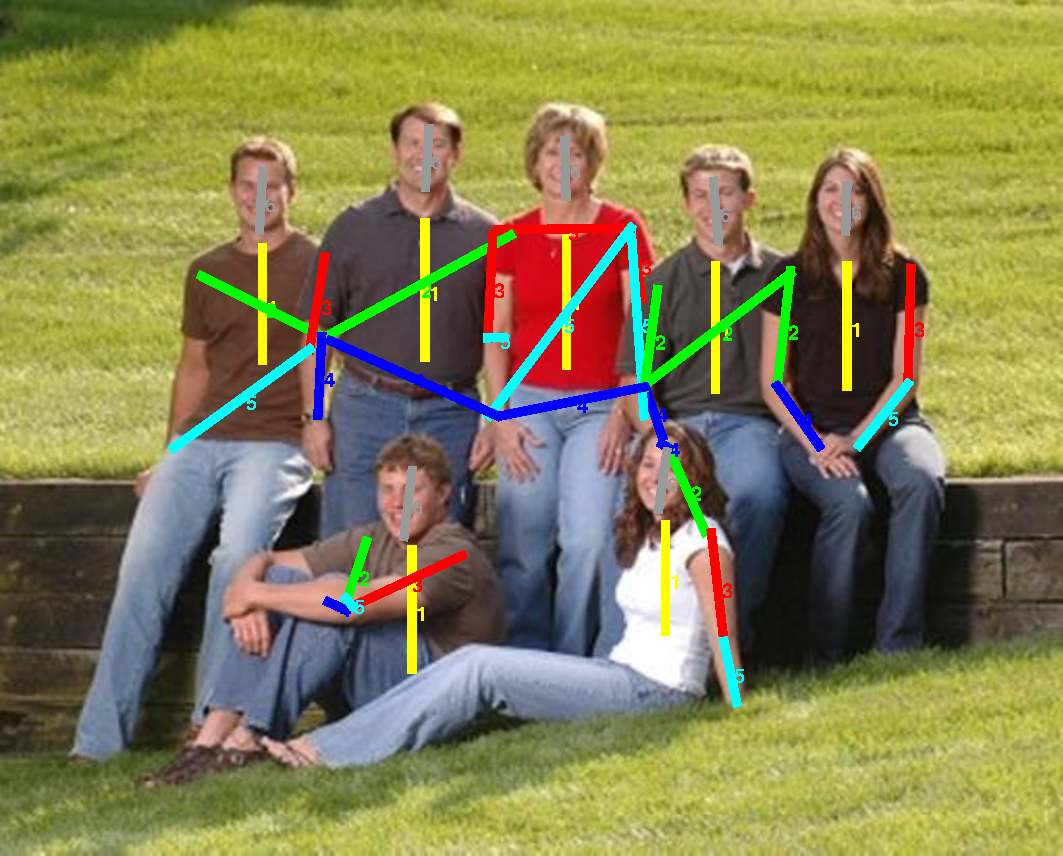
\includegraphics[height=0.150\linewidth]{imgidx_0045_sticks_unary_waf.pdf}&
  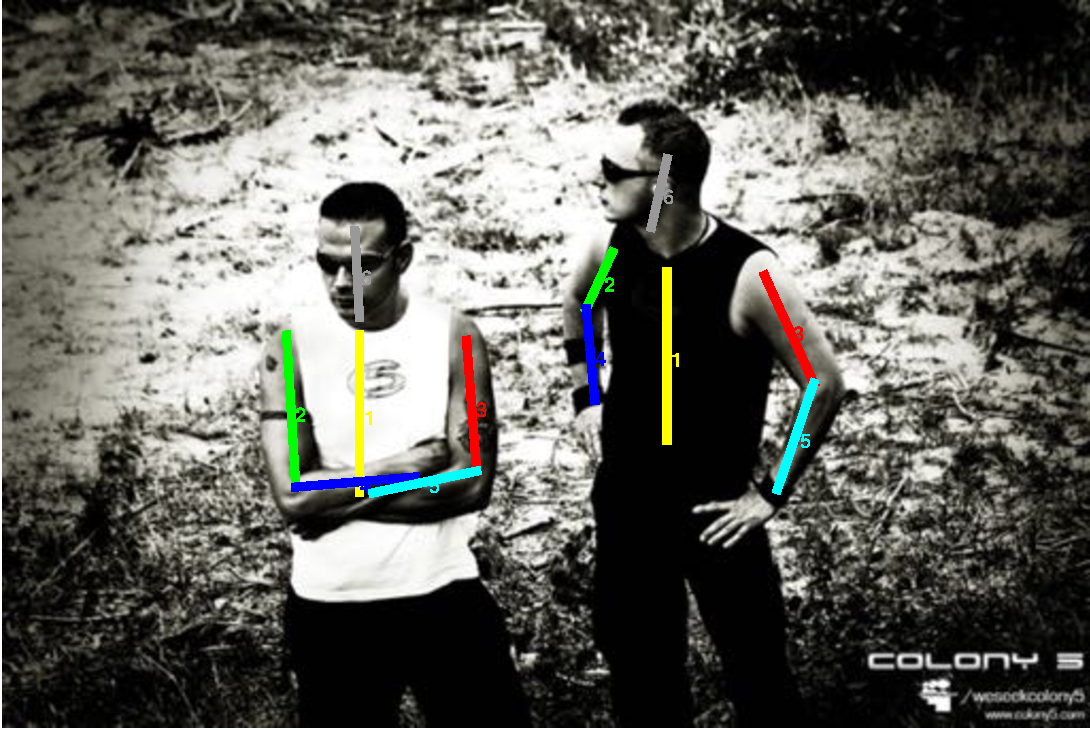
\includegraphics[height=0.150\linewidth]{imgidx_0070_sticks_unary_waf.pdf}&
  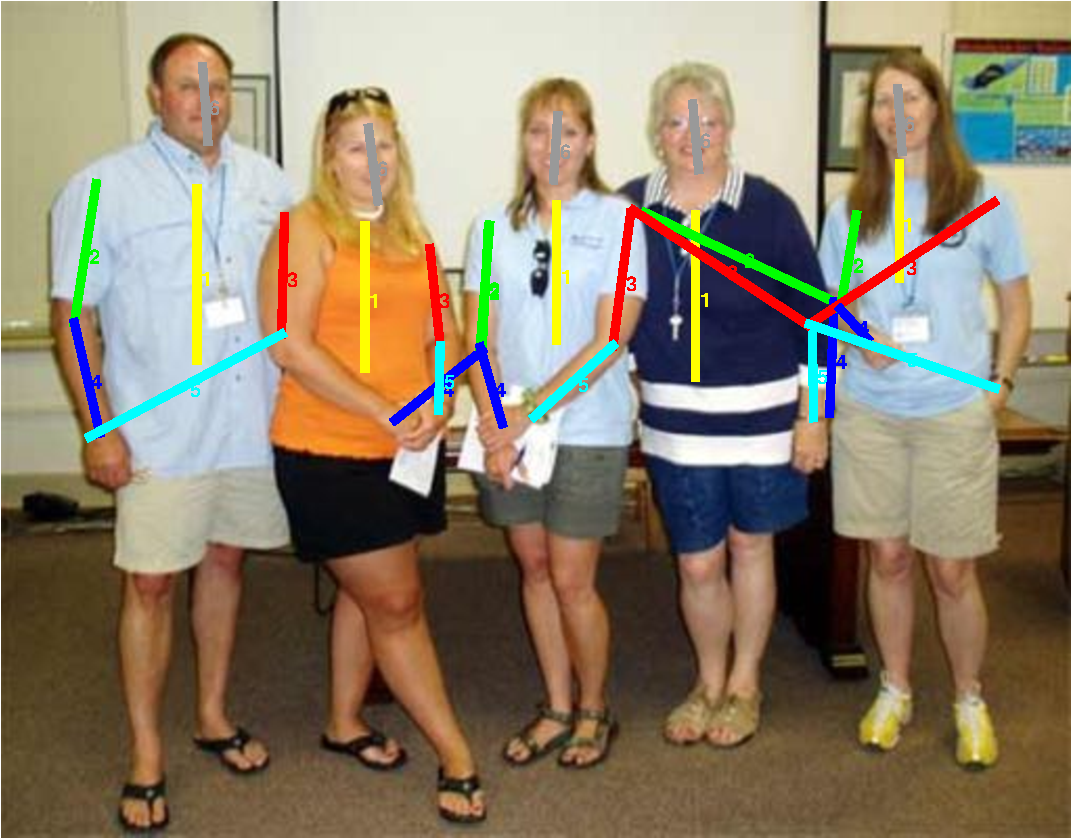
\includegraphics[height=0.150\linewidth]{imgidx_0167_sticks_unary_waf.pdf}&
  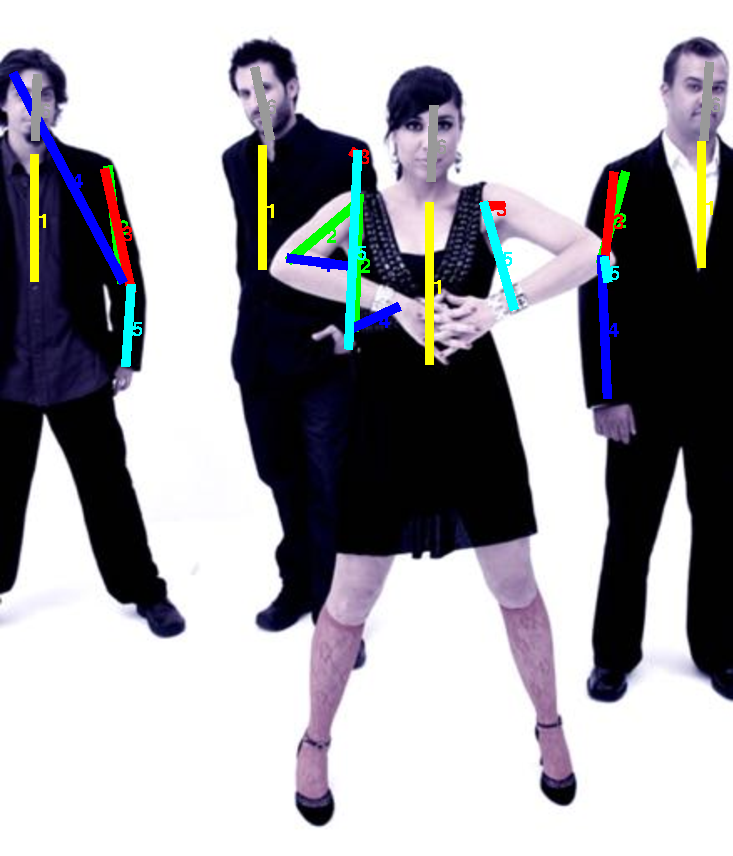
\includegraphics[height=0.150\linewidth]{imgidx_0169_sticks_unary_waf.pdf}\\
  \begin{sideways}\bf \small\quad $\deepcut~\multb$\end{sideways}&
  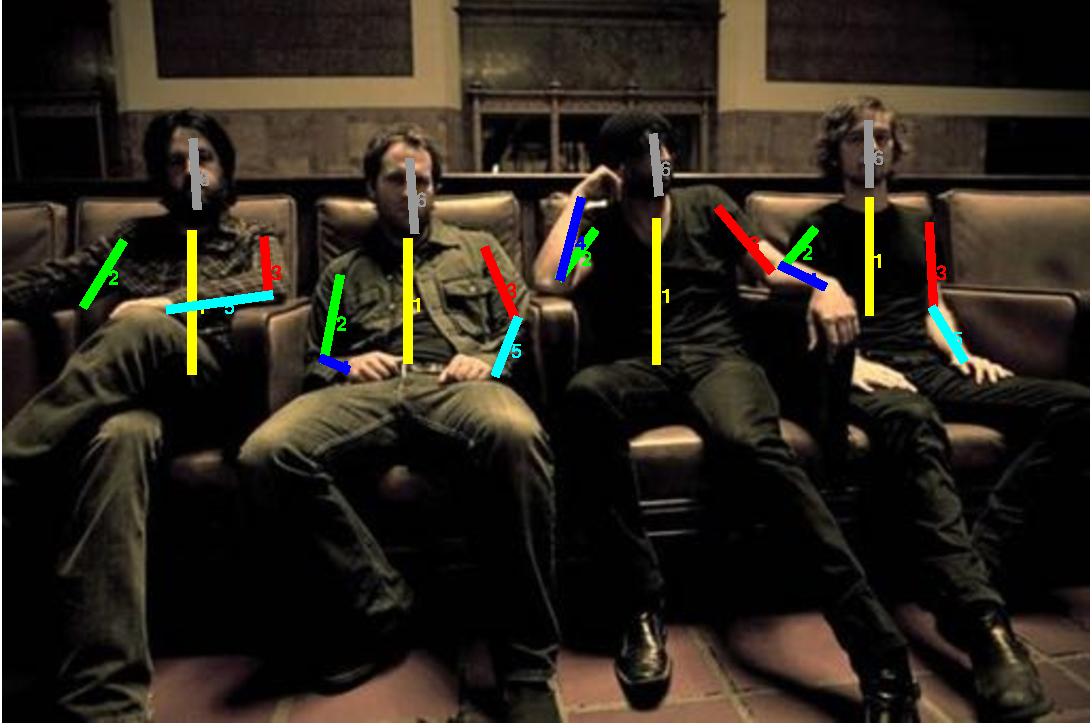
\includegraphics[height=0.150\linewidth]{imgidx_0012_sticks_waf.pdf}&
  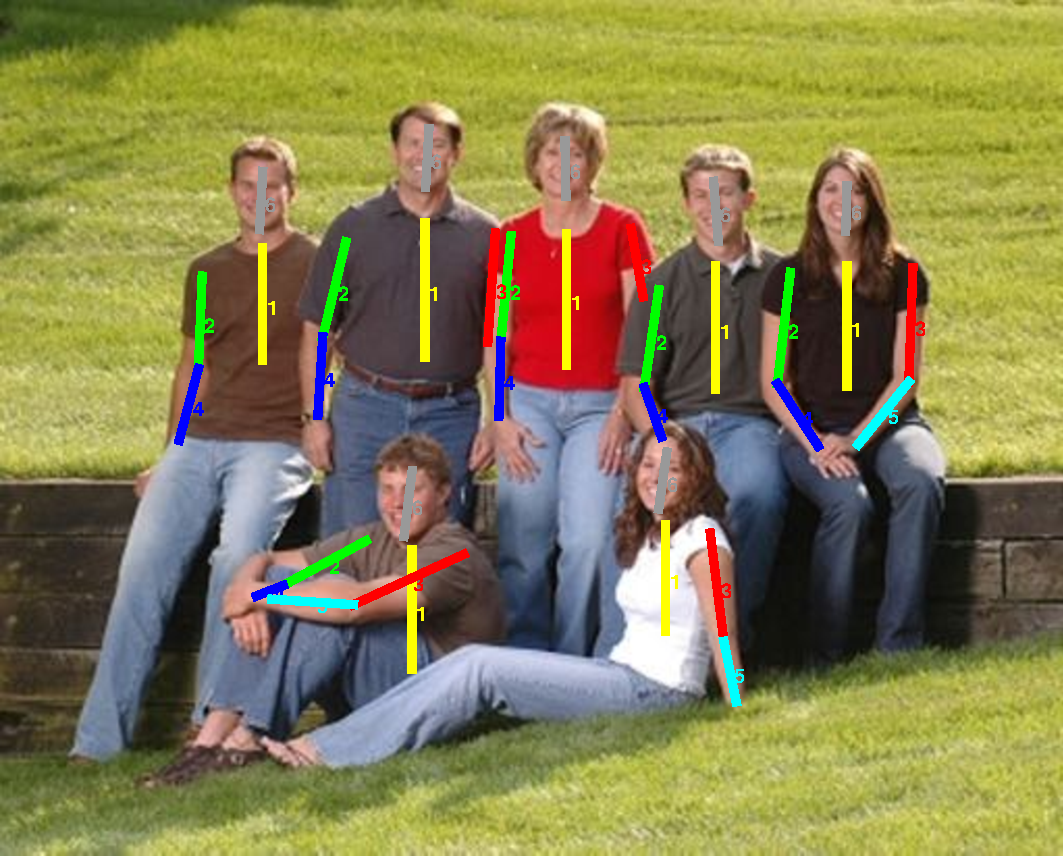
\includegraphics[height=0.150\linewidth]{imgidx_0045_sticks_waf.pdf}&
  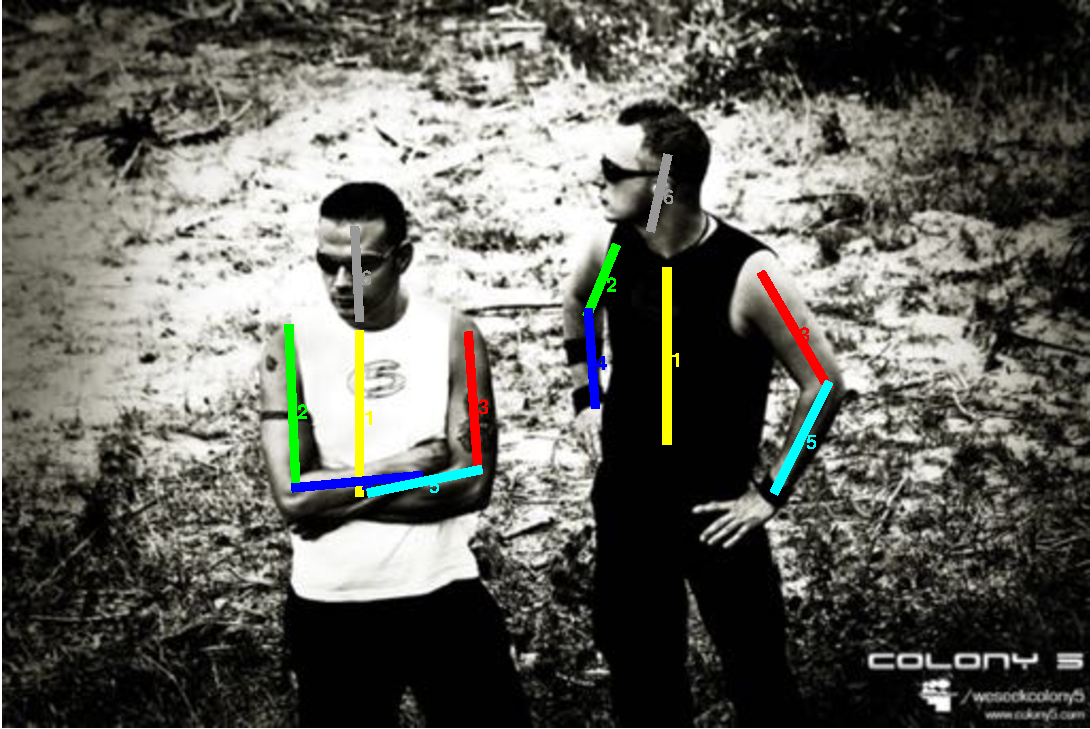
\includegraphics[height=0.150\linewidth]{imgidx_0070_sticks_waf.pdf}&
  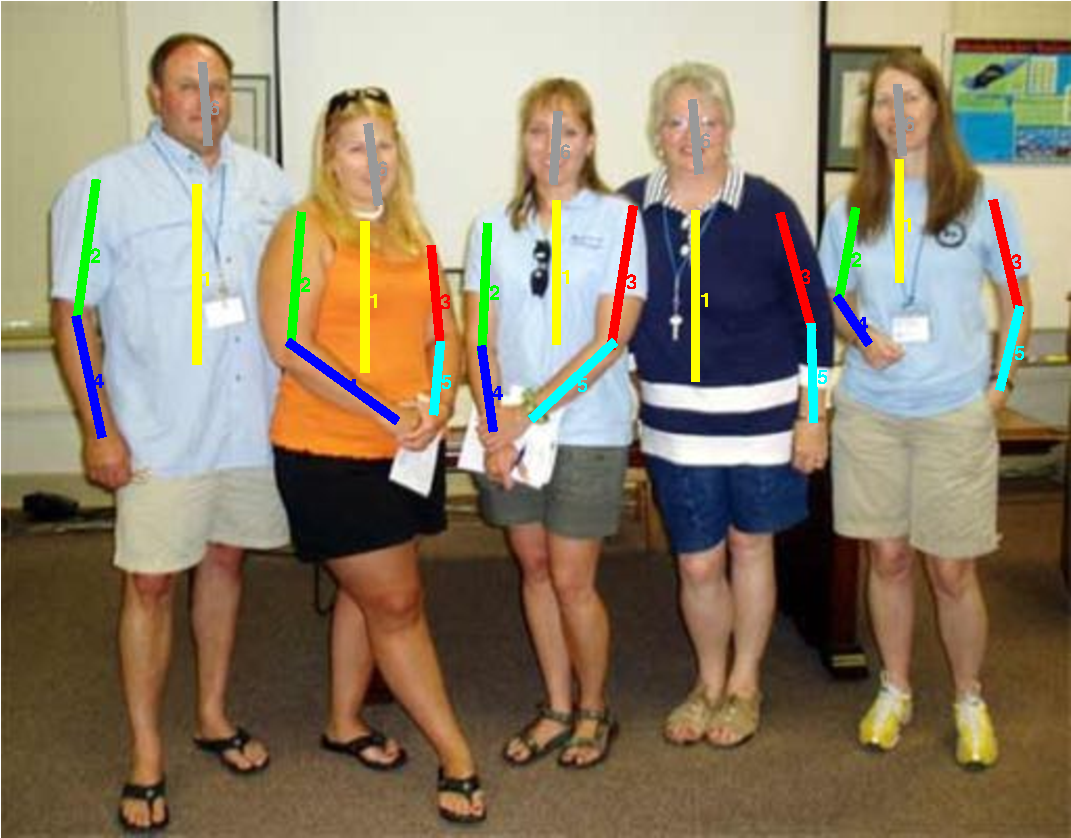
\includegraphics[height=0.150\linewidth]{imgidx_0167_sticks_waf.pdf}&
  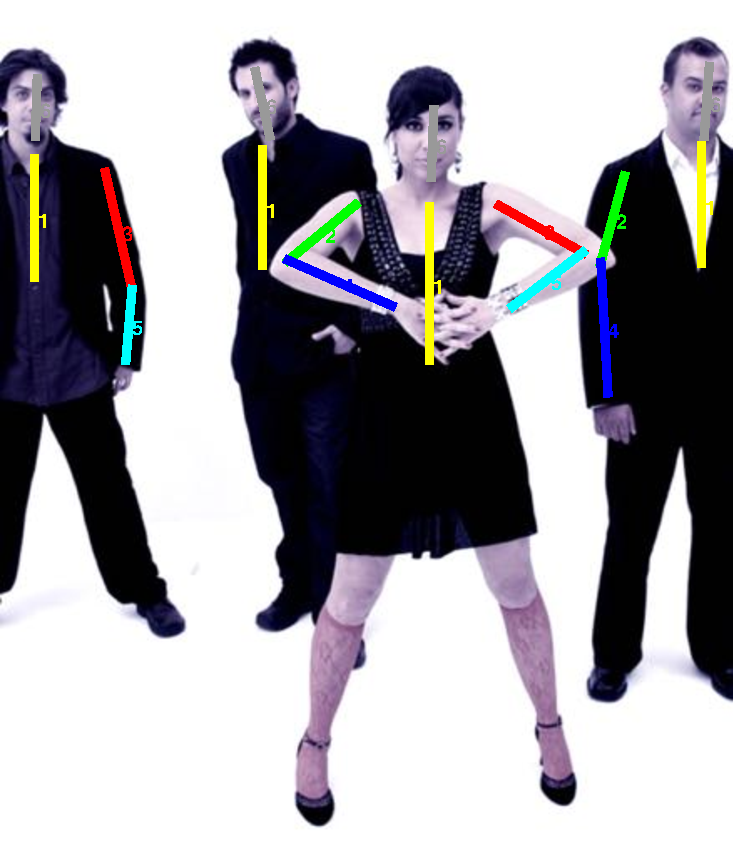
\includegraphics[height=0.150\linewidth]{imgidx_0169_sticks_waf.pdf}\\
  \begin{sideways}\bf \small Chen\&Yuille~\cite{Chen:2015:POC}\end{sideways}&
  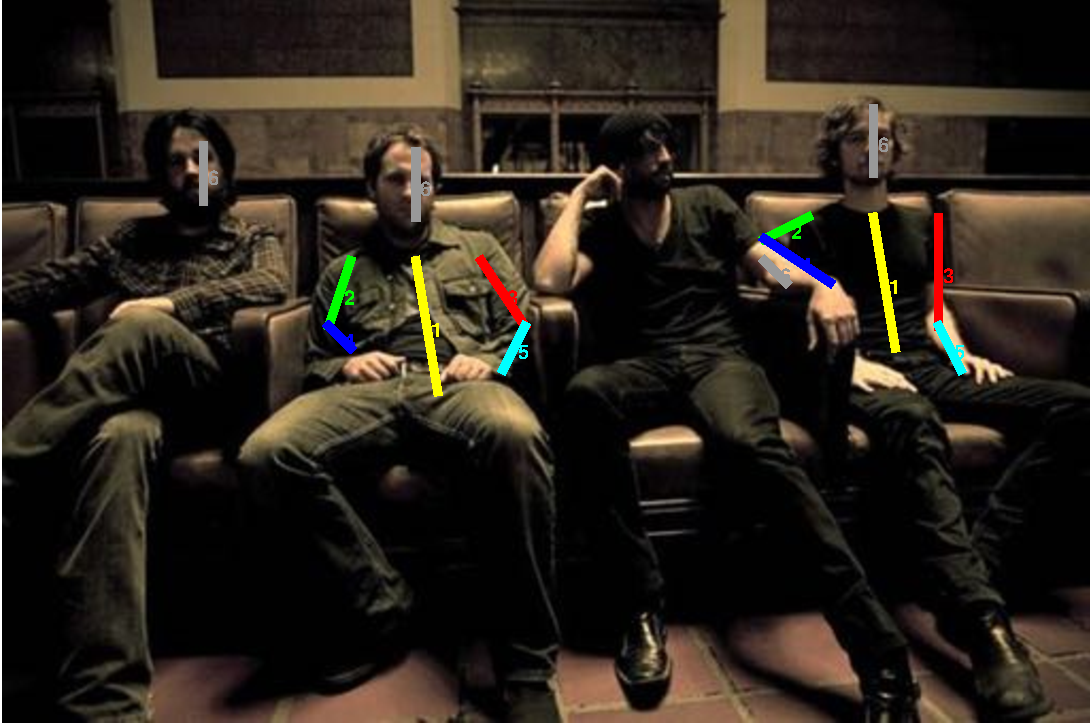
\includegraphics[height=0.150\linewidth]{imgidx_0012_sticks_chen_waf.pdf}&
  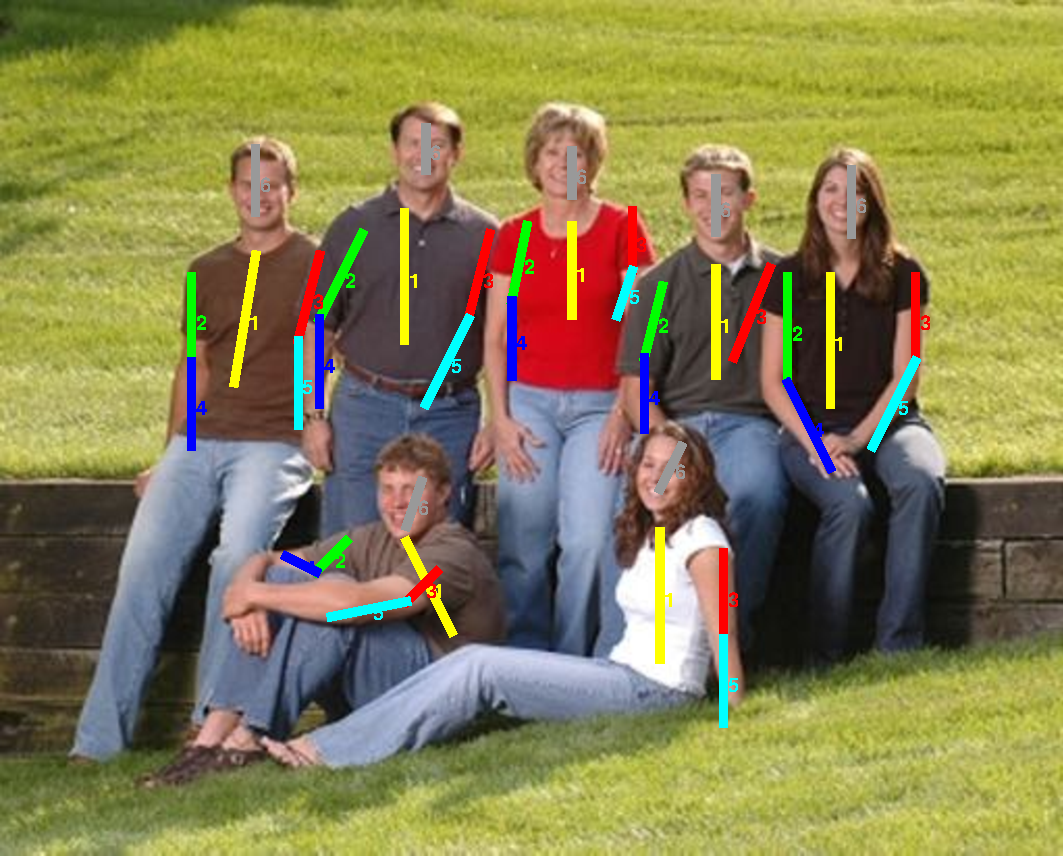
\includegraphics[height=0.150\linewidth]{imgidx_0045_sticks_chen_waf.pdf}&
  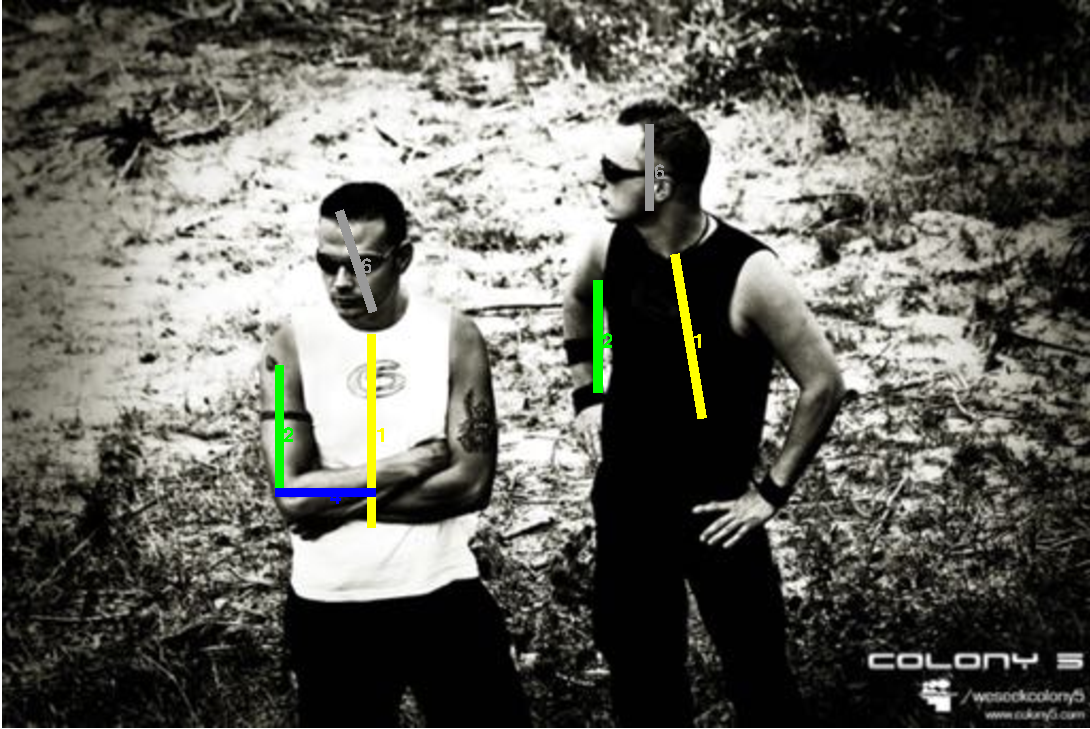
\includegraphics[height=0.150\linewidth]{imgidx_0070_sticks_chen_waf.pdf}&
  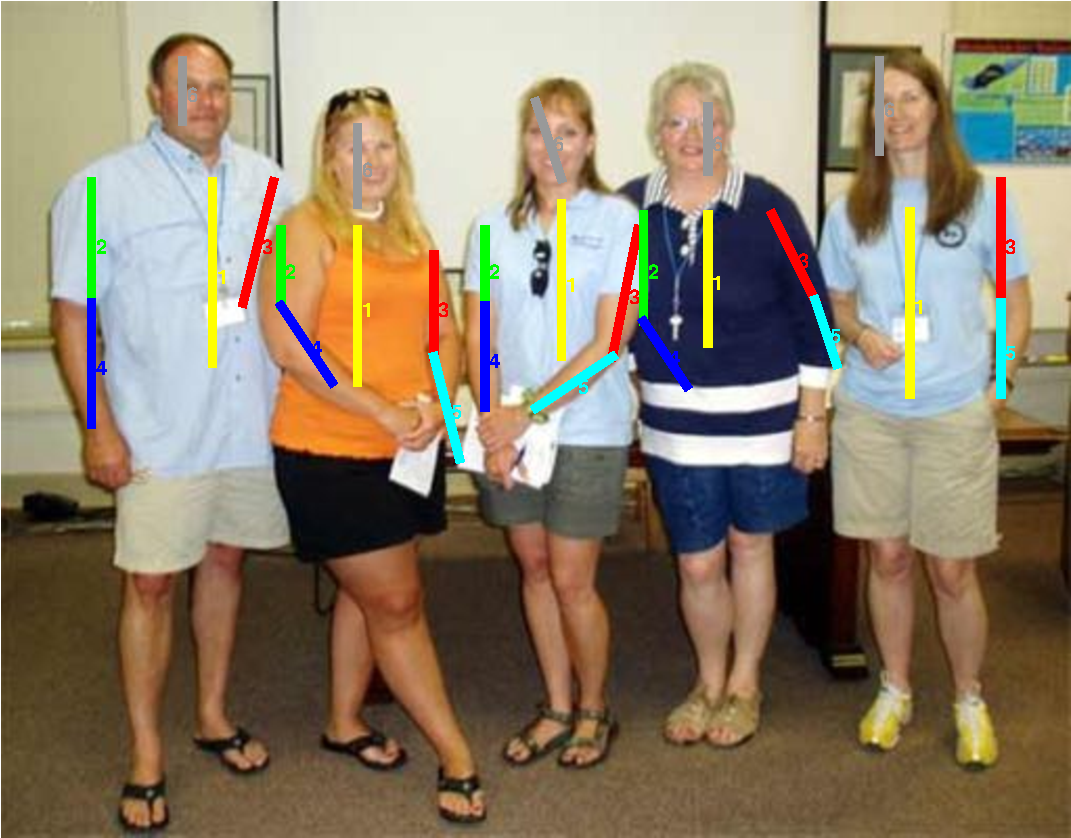
\includegraphics[height=0.150\linewidth]{imgidx_0167_sticks_chen_waf.pdf}&
  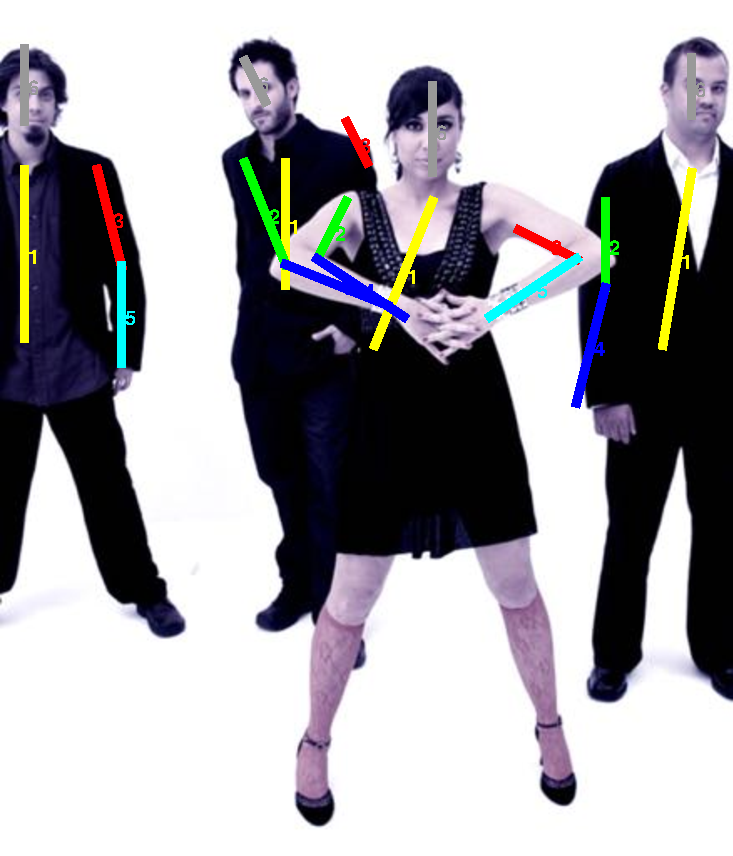
\includegraphics[height=0.150\linewidth]{imgidx_0169_sticks_chen_waf.pdf}\\
  %&1&2&3&4&5\\
 %%  \includegraphics[height=0.275\linewidth]{imgidx_0073_sticks_waf.pdf}&
%%   \includegraphics[height=0.275\linewidth]{imgidx_0073_sticks_unary_waf.pdf}\\
  %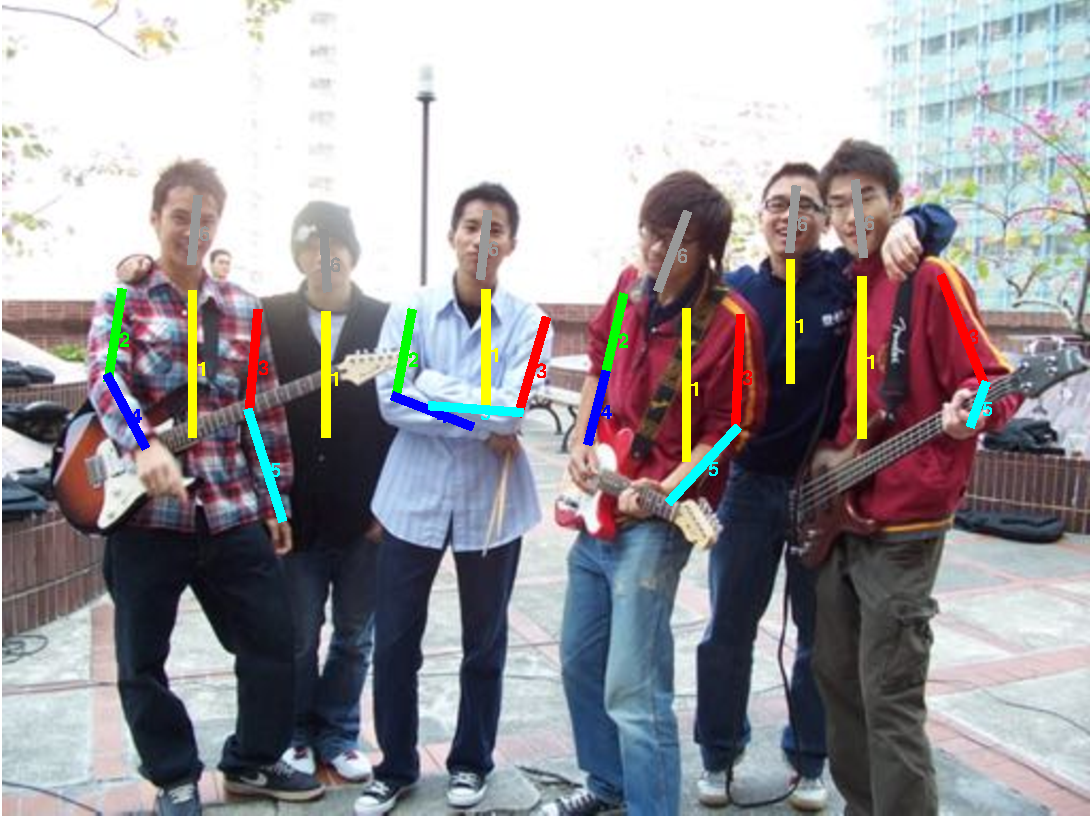
\includegraphics[height=0.275\linewidth]{imgidx_0112_sticks_waf.pdf}&

  %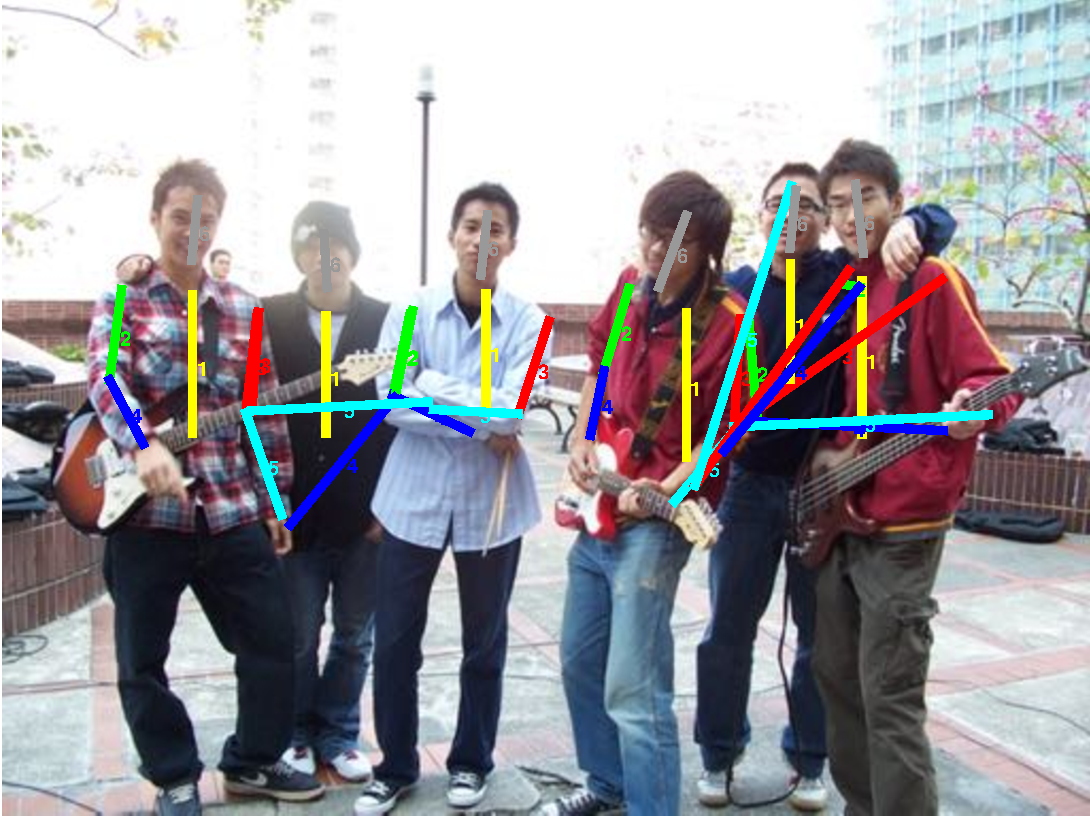
\includegraphics[height=0.275\linewidth]{imgidx_0112_sticks_unary_waf.pdf}\\
%%   \includegraphics[height=0.275\linewidth]{imgidx_0103_sticks_waf.pdf}&
%%   \includegraphics[height=0.275\linewidth]{imgidx_0103_sticks_unary_waf.pdf}\\
  %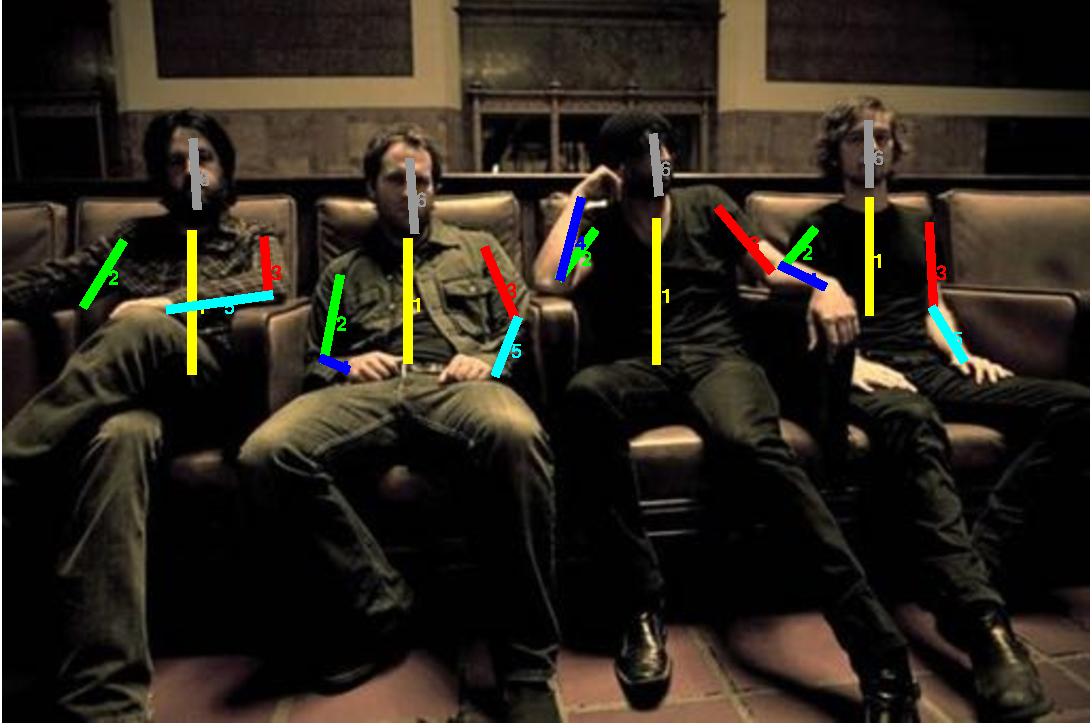
\includegraphics[height=0.275\linewidth]{imgidx_0012_sticks_waf.pdf}&
  %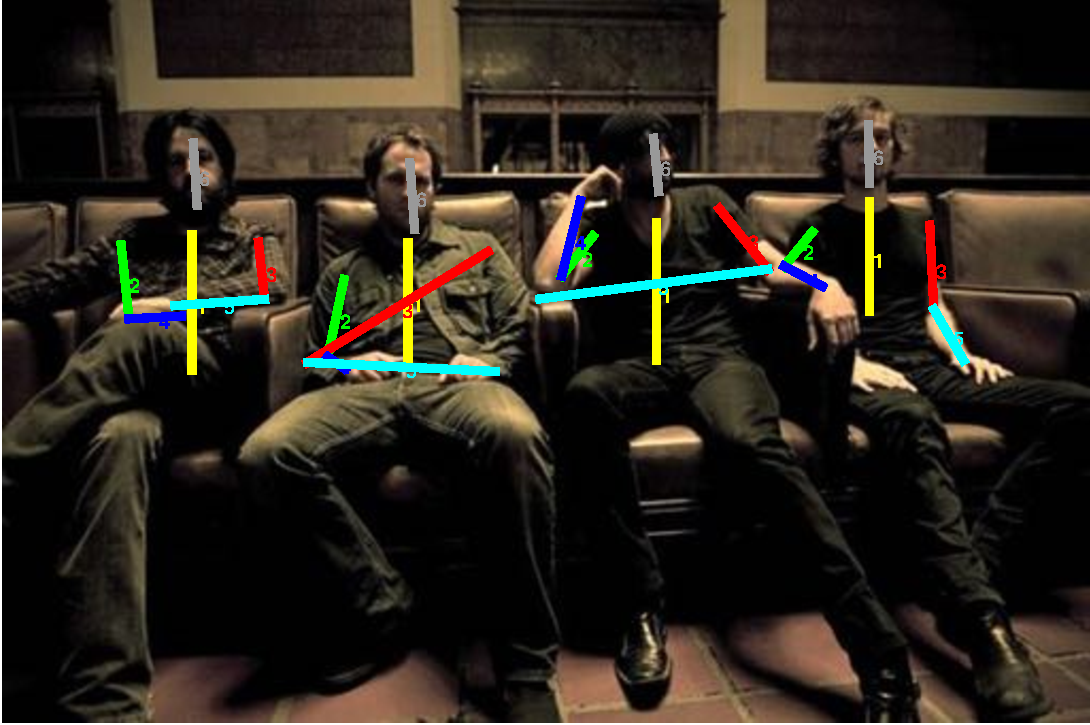
\includegraphics[height=0.275\linewidth]{imgidx_0012_sticks_unary_waf.pdf}\\
%%   \includegraphics[height=0.245\linewidth,width=0.45\linewidth]{imgidx_0026_sticks_waf.pdf}&
%%   \includegraphics[height=0.245\linewidth,width=0.45\linewidth]{imgidx_0026_sticks_unary_waf.pdf}\\
%%   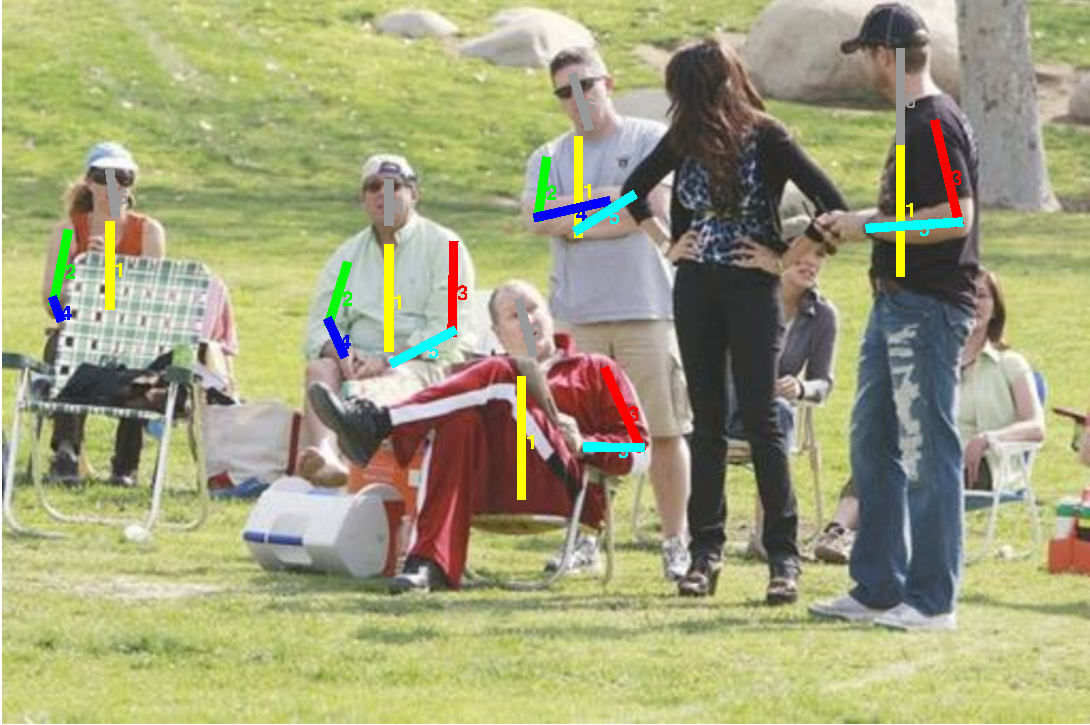
\includegraphics[height=0.245\linewidth,width=0.45\linewidth]{imgidx_0028_sticks_waf.pdf}&
%%   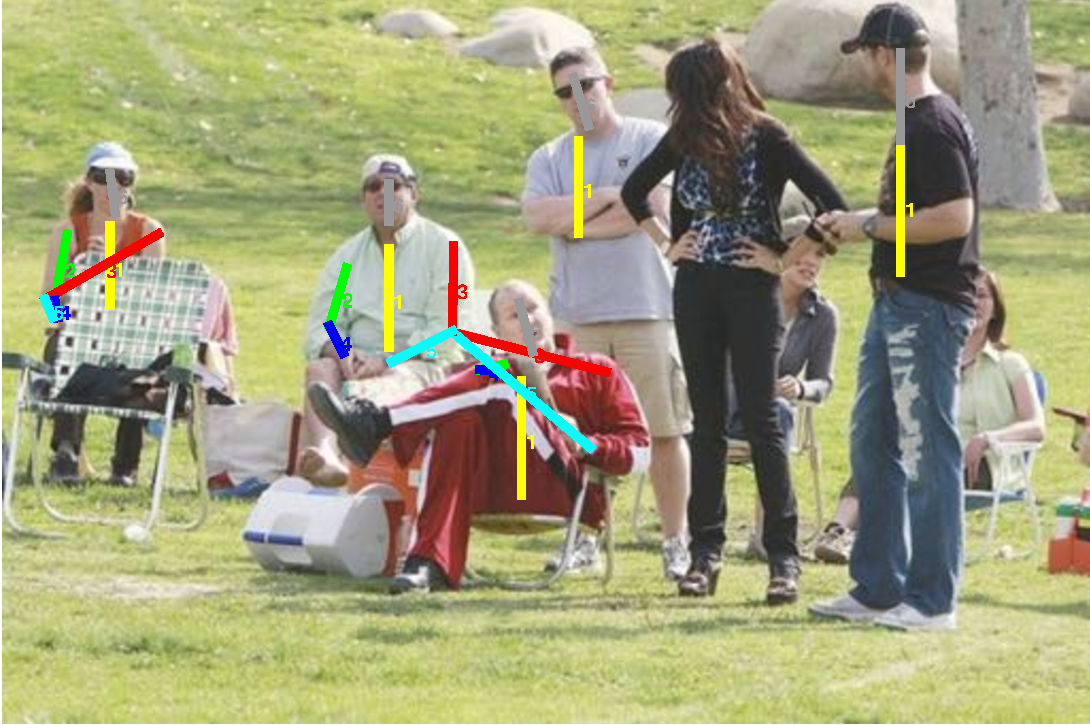
\includegraphics[height=0.245\linewidth,width=0.45\linewidth]{imgidx_0028_sticks_unary_waf.pdf}\\

%%   \includegraphics[height=0.245\linewidth,width=0.45\linewidth]{imgidx_0066_sticks_waf.pdf}&
%%   \includegraphics[height=0.245\linewidth,width=0.45\linewidth]{imgidx_0066_sticks_unary_waf.pdf}\\
%%   \hspace{3.5em}\includegraphics[height=0.275\linewidth]{imgidx_0073_sticks_waf.pdf}&
%%   \hspace{-3.5em}\includegraphics[height=0.275\linewidth]{imgidx_0073_sticks_unary_waf.pdf}\\
%%   \includegraphics[height=0.245\linewidth,width=0.45\linewidth]{imgidx_0104_sticks_waf.pdf}&
%%   \includegraphics[height=0.245\linewidth,width=0.45\linewidth]{imgidx_0104_sticks_unary_waf.pdf}\\

%%   \includegraphics[height=0.245\linewidth,width=0.45\linewidth]{imgidx_0143_sticks_waf.pdf}&
%%   \includegraphics[height=0.245\linewidth,width=0.45\linewidth]{imgidx_0143_sticks_unary_waf.pdf}\\
  %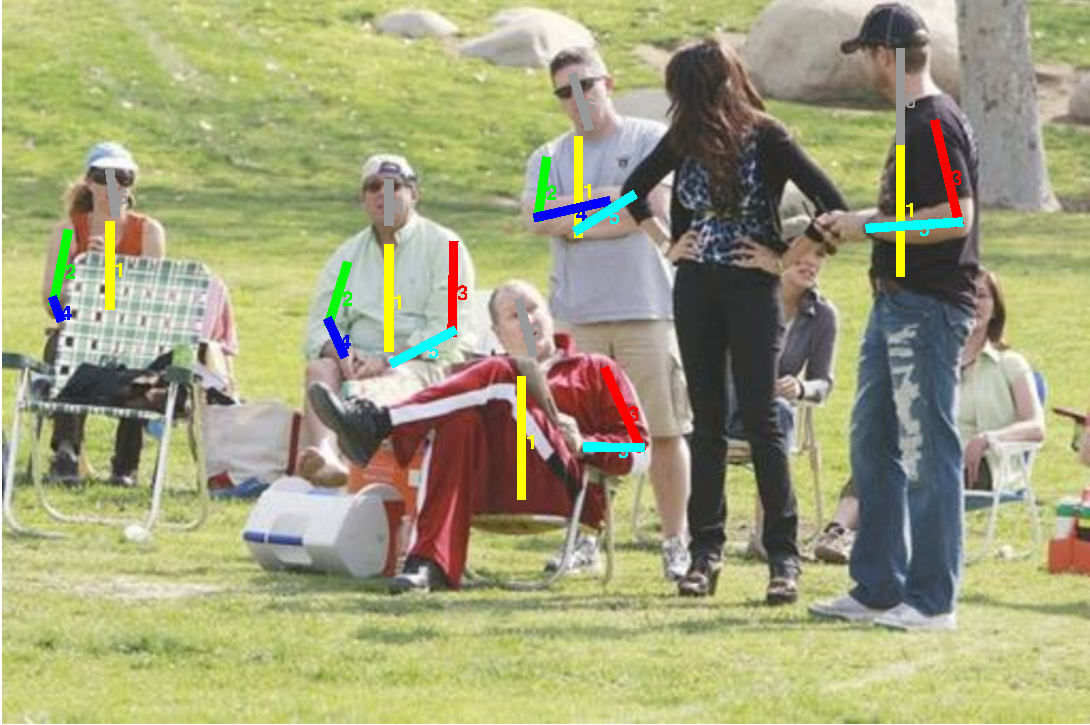
\includegraphics[height=0.275\linewidth]{imgidx_0028_sticks_waf.pdf}&
  %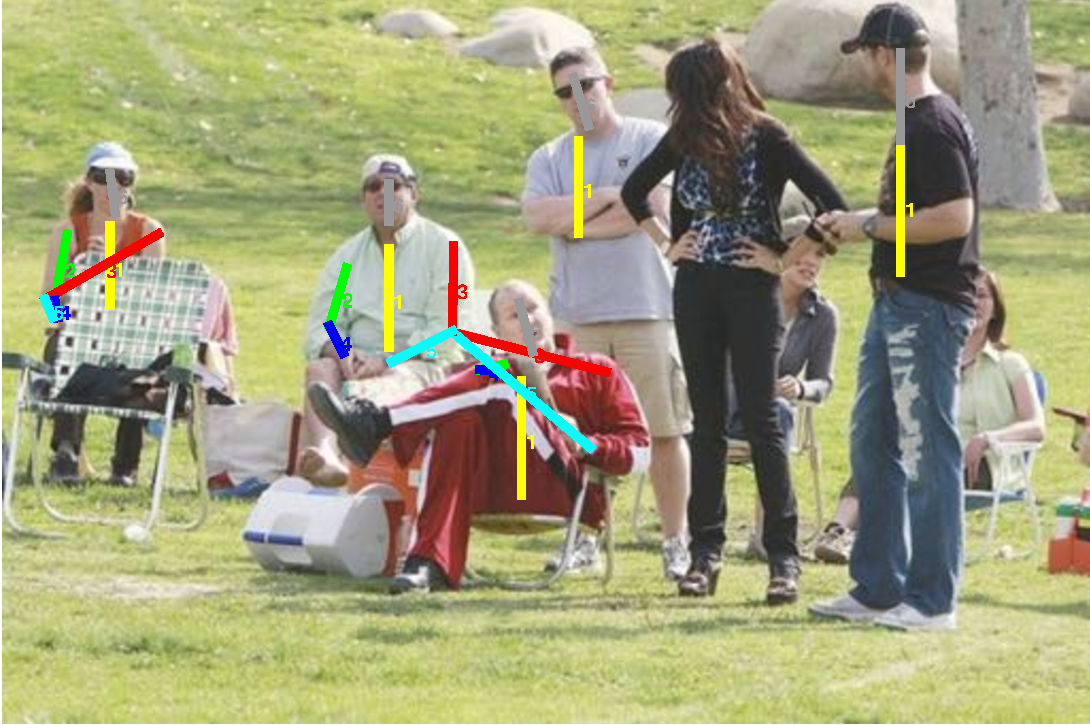
\includegraphics[height=0.275\linewidth]{imgidx_0028_sticks_unary_waf.pdf}\\
  %\includegraphics[height=0.275\linewidth]{imgidx_0001_sticks_waf.pdf}&
  %\includegraphics[height=0.275\linewidth]{imgidx_0001_sticks_unary_waf.pdf}\\
  %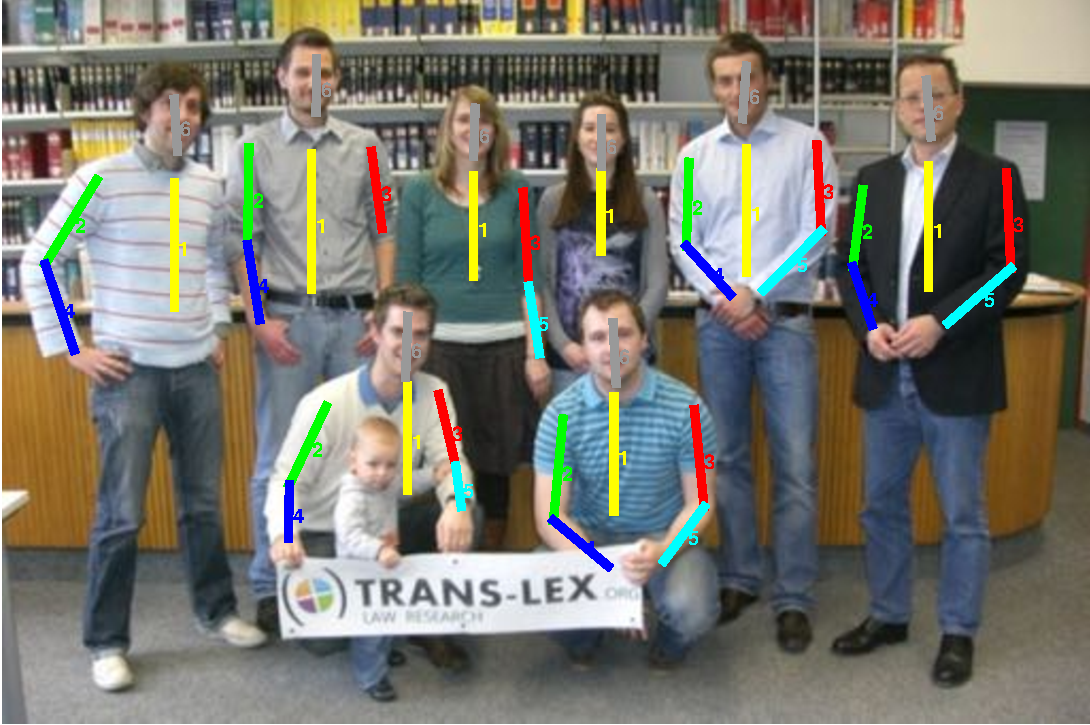
\includegraphics[height=0.275\linewidth]{imgidx_0124_sticks_waf.pdf}&
  %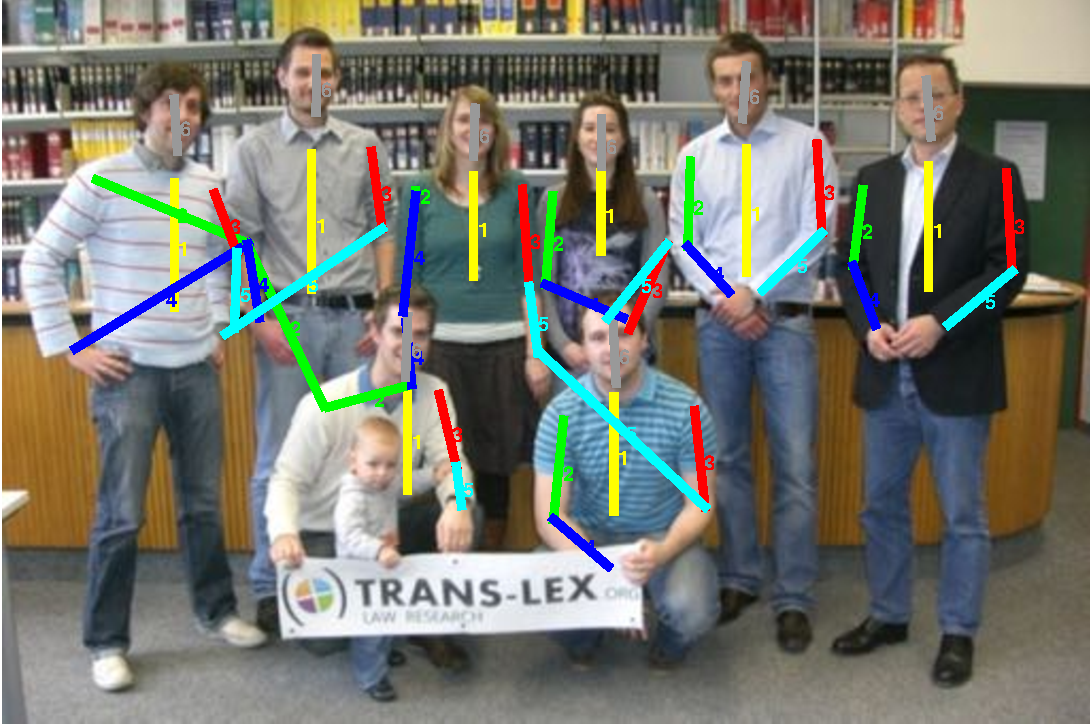
\includegraphics[height=0.275\linewidth]{imgidx_0124_sticks_unary_waf.pdf}\\
% \quad\quad\textbf{Chen\&Yuille}~\cite{Chen:2015:POC}
%\textbf{\deepcut~\multb~\dense} & \quad\textbf{\dense~\detroi}\\
  \end{tabular}
  %\vspace{-0.1em}
\caption{Qualitative comparison of our joint formulation
  $\deepcut~\multb~\dense$ (middle) to the traditional two-stage
  approach $\dense~\detroi$ (top) and the approach of
  Chen\&Yuille~\cite{Chen:2015:POC} (bottom) on WAF dataset. In
  contrast to $\detroi$, $\deepcut~\multb$ is able to disambiguate
  multiple and potentially overlapping persons and correctly assemble
  independent detections into plausible body part configurations. In
  contrast to ~\cite{Chen:2015:POC}, $\deepcut~\multb$ can better
  predict occlusions (image 2 person $1-4$ from the left, top row;
  image 4 person 1, 4; image 5, person 2) and better cope with strong
  articulations and foreshortenings (image 1, person 1, 3; image 2
  person 1 bottom row; image 3, person 1-2). See
  Appendix~\ref{sec:supplemental:waf} for more examples.
  %See supplementary material for more examples.
    %, but may fail                                                                                                                                                                                                                           
    %due to missing recall of part detection set (row 4 person 2, row 5                                                                                                                                                                       
    %person 3, 4).                                                                                                                                                                                                                            
  }
   \vspace{-1.0em}
  \label{fig:qualitative_waf_2}
\end{figure*}

%\begin{figure}
  \centering
  \begin{tabular}{c c c }
  \includegraphics[height=0.245\linewidth,width=0.45\linewidth]{figures/waf/imgidx_0005_sticks.pdf}&
  \includegraphics[height=0.245\linewidth,width=0.45\linewidth]{figures/waf/imgidx_0005_sticks_chen.pdf}\\
  \includegraphics[height=0.245\linewidth,width=0.45\linewidth]{figures/waf/imgidx_0007_sticks.pdf}&
  \includegraphics[height=0.245\linewidth,width=0.45\linewidth]{figures/waf/imgidx_0007_sticks_chen.pdf}\\
  \includegraphics[height=0.245\linewidth,width=0.45\linewidth]{figures/waf/imgidx_0014_sticks.pdf}&
  \includegraphics[height=0.245\linewidth,width=0.45\linewidth]{figures/waf/imgidx_0014_sticks_chen.pdf}\\

  \includegraphics[height=0.245\linewidth,width=0.45\linewidth]{figures/waf/imgidx_0053_sticks.pdf}&
  \includegraphics[height=0.245\linewidth,width=0.45\linewidth]{figures/waf/imgidx_0053_sticks_chen.pdf}\\

  \includegraphics[height=0.245\linewidth,width=0.45\linewidth]{figures/waf/imgidx_0063_sticks.pdf}&
  \includegraphics[height=0.245\linewidth,width=0.45\linewidth]{figures/waf/imgidx_0063_sticks_chen.pdf}\\
  \includegraphics[height=0.245\linewidth,width=0.45\linewidth]{figures/waf/imgidx_0097_sticks.pdf}&
  \includegraphics[height=0.245\linewidth,width=0.45\linewidth]{figures/waf/imgidx_0097_sticks_chen.pdf}\\
  \includegraphics[height=0.245\linewidth,width=0.45\linewidth]{figures/waf/imgidx_0119_sticks.pdf}&
  \includegraphics[height=0.245\linewidth,width=0.45\linewidth]{figures/waf/imgidx_0119_sticks_chen.pdf}\\
  \includegraphics[height=0.245\linewidth,width=0.45\linewidth]{figures/waf/imgidx_0135_sticks.pdf}&
  \includegraphics[height=0.245\linewidth,width=0.45\linewidth]{figures/waf/imgidx_0135_sticks_chen.pdf}\\
  \includegraphics[height=0.245\linewidth,width=0.45\linewidth]{figures/waf/imgidx_0174_sticks.pdf}&
  \includegraphics[height=0.245\linewidth,width=0.45\linewidth]{figures/waf/imgidx_0174_sticks_chen.pdf}\\
  
  \end{tabular}
  \vspace{-0.1em}
  \caption{ \textcolor{red}{Qualitative comparison on "We are the family" dataset.  Images from Chen and Yullie paper. {\it First
        column}: Results by our approach. {\it Second column}: corresponding results shown in \cite{Chen:2015:POC} .}
  } 
    \vspace{-1.2em}
  \label{fig:qualitative_waf}
\end{figure}


\myparagraph{Results on MPII Multi-Person.}
%% We first describe the way
%% we compute \detroi~and~\gtroi~and then present the results.
%\noindent $\detroi$.
Obtaining a strong detector of highly articulated people having strong
occlusions and truncations is difficult. We employ a neck detector as
a person detector as it turned out to be the most reliable part.
%Optimal IoU-based non-maximum suppression and detection thresholds were
%selected using the training set.
%% , which results
%% in detection performance of 76.7\% AP on the test set, the highest
%% among the part detectors.
Full body bounding box is created around a neck detection and used as~\detroi.
%Then we non-uniformly extend detection bounding box while also taking
%the scale into account
%%  such that it has a size of
%% the upright person. This region is then used
%and use this box as \detroi. 
\gtroi s were provided by the authors~\cite{andriluka14cvpr}.
%% \noindent We now define four baselines based on the \emph{ROI}:
%% \noindent\emph{Unaries from $\detroi$} ($\undetroi$).
%% We extract a single highest scoring location for each body part
%% falling inside the $\detroi$.
%% \noindent\emph{Unaries from $\gtroi$} ($\ungtroi$).
%% Same as above but using the $\gtroi$.
%% \noindent\emph{Chen\&Yuille~\cite{chen14nips} on $\detroi$} ($\cydetroi$).
%% We perform single person pose estimation using the state of the art method of~\cite{chen14nips} applied to $\detroi$
%% crops.
%$\cygtroi$).
As the $\multb$ approach~\cite{Chen:2015:POC} is not public, we
compare to $\singb$ state-of-the-art method~\cite{chen14nips} applied
to $\gtroi$ image crops.

Results are shown in
Tab.~\ref{tab:multicut:mpii-multi}. 
%% \rcnn~$\detroi$ achieves $47.1$\%
%% AP. 
$\deepcut~\multb~\rcnn$ improves over $\rcnn~\detroi$ by 4.3\%
achieving 51.4\% AP. The largest differences are observed for the
ankle, knee, elbow and wrist, as those parts benefit more from the
connections to other parts. 
%We evaluate the performance of the
%$\multbu$ model that includes upper body parts
%only. 
$\deepcut~\multbu~\rcnn$ using upper body parts only slightly improves
over the full body model when compared on common parts (60.5 vs 58.2\%
AP). Similar tendencies are observed for $\dense$s, though improvements
of $\multbu$ over $\multb$ are more significant.
%% with two differences: 1) similar to the
%% other datasets the performance by $\deepcut~\dense$ models is higher
%% compared to $\deepcuts~\rcnn$; and 2) the performance of
%% ($\deepcuts~\multbu~\rcnn$)~is much better compared to $\multb$.%, due
%% %to better wrist estimation. %\todo{why?}

All $\deepcuts$ outperform $\cygtroi$, partially due to stronger part
detectors compared to~\cite{chen14nips}
(c.f. Tab.~\ref{tab:multicut:lsp}). Another reason is that $\cygtroi$
does not model body part occlusion and truncation always predicting
the full set of parts, which is penalized by the AP measure. In
contrast, our formulation allows to deactivate the part hypothesis in
the initial set of part candidates thus effectively performing
non-maximum suppression. In $\deepcuts$ part hypotheses are suppressed
based on the evidence from all other body parts making this process
more reliable.

%% \myparagraph{Performance analysis by the number of people.}  In order
%% to better understand the strengths and weaknesses of our multi-person
%% models, we analyze their performance on as a function of the number of
%% people in the image. We consider the images containing only $2$, $3$,
%% $4$, or at least $5$ people and compare the results by multi-person
%% models $\mult$ and $\multu$ to unaries only ($\undetroi$). The results
%% are shown in Tab.~\ref{tab:number-of-people}. It shows that in
%% each case the performance drops with the increased number of
%% people. We observe that the overall performance drop by $\mult$ is
%% much lower compared to $\undetroi$ for which performance is halved
%% (-4.7 vs -13.3\% AP). The difference between both approaches increases
%% with the increased number of people, reaching 10\% AP in case of $\ge$
%% 5 people. This underlines the advantages of our model that jointly
%% reasons about the number of people and part assignment. It can be seen
%% that $\multu$ is even more robust to the increasing number of people
%% (-2.6\% AP). In this case, the least performance drop is observed for
%% the head and shoulders. Similar to the results on the full set,
%% $\multu$ outperforms $\mult$ for all upper body parts. The difference
%% is most pronounced in case of $\ge$ 5 people (37.0 vs 30.4\% AP). This
%% suggests that less reliable detections of the frequently occluded
%% lower body parts and their connections to other parts weaken the
%% overall performance of the full body model. We envision that stronger
%% spatial and appearance terms for the lower body parts, as well as
%% larger number of initial detections should improve the performance the
%% full body model.

%%\renewcommand{\tabcolsep}{0.15cm}
\tabcolsep 1.0pt
\begin{table}[tbp]
 \scriptsize
  \centering
  \begin{tabular}{@{} l c ccc ccc cc@{}}
    \toprule
    Setting& Head   & Sho  & Elb & Wri & Hip & Knee & Ank & Up & Full\\
           &        &           &       &       &     &      &       & body  & body \\
    \midrule
    oracle 2000& 98.8  & 98.8  & 97.4  & 96.4  & 97.4  & 98.3 & 97.7 & 97.8 & 84.0\\


    \midrule
    DPM scale 1& 48.8  & 25.1  & 14.4  & 10.2  & 13.6  & 21.8 & 27.1 & 23.0 & 13.6\\

    \midrule    
    %AlN s1 lr.001(80k) 140k IoU.5 & 82.2  & 67.0  & 49.6  & 45.4  & 53.1  & 52.9 & 48.2 & 56.9 & 35.9 \\
AlexNet scale 1 & 82.2  & 67.0  & 49.6  & 45.4  & 53.1  & 52.9 & 48.2 & 56.9 & 35.9 \\


    AlexNet scale 4 & 85.7  & 74.4  & 61.3  & 53.2  & 64.1  & 63.1 & 53.8 & 65.1 & 39.0 \\


    AlexNet scale 4, \textbf{lr 0.003, lr step 160k, \# iter 240k}, IoU pos/neg 0.5 & 87.0  & 75.1  & 63.0  & 56.3  & 67.0  & 65.7 & 58.0 & 67.4 & 40.8\\


    AlexNet scale 4, lr 0.003, lr step 160k, \# iter 240k, \textbf{IoU pos/neg 0.4} & 87.5  & 76.7  & 64.8  & 56.0  & 68.2  & 68.7 & 59.6 & 68.8 & 40.9\\


    AlexNet scale 4, lr 0.003, lr step 160k, \# iter 240k, IoU pos/neg 0.4, \textbf{data augment} & 87.8  & 77.8  & 66.0  & 58.1  & 70.9  & 66.9 & 59.8 & 69.6 & 42.3\\


    %AlN s4 lr.004(320k) 1M IoU.4 aug& 88.1  & 79.3  & 68.9  & 62.6  & 73.5  & 69.3 & 64.7 & 72.4 & 44.6 \\
\quad + optimal params & 88.1  & 79.3  & 68.9  & 62.6  & 73.5  & 69.3 & 64.7 & 72.4 & 44.6 \\


    AlN lr0.004 \textbf{(500k) 2M} sc4 IoU0.4 augm& 88.4  & 79.7  & 69.2  & 62.1  & 73.3  & 72.0 & 65.6 & 70.3 & 72.9 \\


    \quad\quad + finetune LSP & 92.9  & 81.0  & 72.1  & 66.4  & 80.6  & 77.6 & 75.0 & 77.9 & 51.6\\


    \midrule
    %VGG s4 lr.003(160k) 320k IoU.4 aug& 91.0  & 84.2  & 74.6  & 67.7  & 77.4  & 77.3 & 72.8 & 77.9 & 50.0 \\
VGG scale 4 optimal params & 91.0  & 84.2  & 74.6  & 67.7  & 77.4  & 77.3 & 72.8 & 77.9 & 50.0 \\

 
    %VGG lr0.004 (160k) \textbf{520M} sc4 IoU0.4 augm& 91.1  & 84.6  & 75.2  & 69.1  & 78.2  & 77.8 & 72.9 & 76.3 & 78.4\\


    %\quad + finetune LSP lr0.0005 (10k) 40k & \textbf{95.4}  & \textbf{86.5}  & \textbf{77.8}  & \textbf{74.0}  & \textbf{84.5}  & \textbf{78.8} & \textbf{82.6} & \textbf{82.8} &\textbf{57.0}\\
\quad + finetune LSP & \textbf{95.4}  & \textbf{86.5}  & \textbf{77.8}  & \textbf{74.0}  & \textbf{84.5}  & \textbf{78.8} & \textbf{82.6} & \textbf{82.8} &\textbf{57.0}\\


    \quad\quad + \textit{no} bbox reg& 94.1  & 85.1  & 76.8  & 72.8  & 81.2  & 81.4 & 77.5 & 78.3 & 81.3 \\


    \bottomrule
  \end{tabular}
  \caption[]{Unary only performance (PCK) of adapted Fast R-CNN on the LSP (Person-Centric) dataset.}
    \vspace{-0.5em}
  \label{tab:rcnn}
\end{table}

%\renewcommand{\tabcolsep}{0.15cm}
\tabcolsep 1.5pt
\begin{table}[tbp]
 \scriptsize
  \centering
  \begin{tabular}{@{} l c ccc ccc cc@{}}
    \toprule
    Setting& Head   & Sho  & Elb & Wri & Hip & Knee & Ank & UBody & FBody \\
    \midrule
    %% Fast R-CNN \detroi~\textcolor{red}{76} & 62.0  & 55.4  & 42.6  & 29.5  & 33.4  & 25.3 & 16.9 & 47.4 & 38.5 \\


%%     Fast R-CNN \multb~\textcolor{red}{76}& 63.5  & 56.5  & 44.2  & 30.1  & 37.4  & 26.6 & 25.5 & 48.6 & 41.1 \\


%%     Fast R-CNN \detroi~\textcolor{red}{840}& 64.5  & 58.5  & 39.7  & 27.4  & - & - & - & 47.5 & - \\


%%     Fast R-CNN \multbu~\textcolor{red}{840}& 66.4  & 60.1  & 44.9  & 30.5  & -  & - & - & 50.5 & - \\


%%     \midrule
%%     Fast R-CNN \gtroi~\textcolor{red}{76}& 64.6  & 58.1  & 46.1  & 35.9  & 36.6  & 28.6 & 21.4 & 51.2 & 42.2 \\


%%     Fast R-CNN \gtroi~\textcolor{red}{840}& 68.1  & 60.6  & 45.8  & 37.0  & -  & - & - & 52.9 & - \\


%%     \midrule
%%     Dense \detroi~\textcolor{red}{408} & 67.5  & 64.8  & 50.5  & 36.6  & 48.3  & 37.8 & 26.7 & 54.8 & 47.9 \\

%%     Dense \multb~\textcolor{red}{408} & 68.1  & 64.4  & 50.7  & 35.2  & 49.5  & 39.0 & 28.8 & 54.6 & 48.4  \\

%%     Dense \multbu~\textcolor{red}{522} & 76.2  & 68.8  & 58.6  & 44.7  & -  & - & - & 62.1 & - \\
Dense \gtroi~\multbu~\textcolor{red}{522} & 78.4  & 71.4  & 60.3  & 51.7  & -  & - & - & 65.4 & - \\

%%     \midrule
%%     Dense \gtroi~\textcolor{red}{408}& 74.5  & 69.7  & 59.3  & 48.5  & 51.8  & 47.5 & 44.9 & 63.0 & 57.0 \\


%%     \textcolor{red}{103 images}\\
%%     Fast R-CNN \detroi& 72.0  & 68.4  & 55.2  & 35.8  & 47.1  & 35.5 & 22.0 & 57.8 & 48.6 \\


%%     Fast R-CNN \multb& 73.5  & 68.6  & 58.0  & 39.7  & 49.6  & 39.8 & 26.9 & 60.0 & 51.5 \\


%%     Fast R-CNN \multbu& 74.6  & 71.4  & 61.3  & 39.5  & -  & - & - & 61.7 & - \\


%%     \midrule
%%     Dense \detroi& 78.2  & 75.9  & 61.6  & 43.7  & 53.1  & 41.5 & 33.0 & 64.8 & 55.9 \\


%%     Dense \multb& 76.2  & 76.1  & 62.0  & 38.4  & 57.3  & 48.0 & 33.3 & 63.2 & 56.4 \\


%%     Dense \multbu& 82.8  & 80.4  & 67.6  & 55.8  & -  & - & - & 71.7 & - \\


%%     \midrule
%%     Fast R-CNN \gtroi& 72.9  & 67.5  & 57.1  & 43.4  & 50.1  & 44.3 & 38.2 & 60.2 & 53.8 \\


%%     Dense \gtroi& 75.8  & 77.2  & 64.6  & 52.6  & 55.9  & 47.7 & 45.0 & 67.6 & 60.4 \\

 

%%    \textcolor{red}{162 images}\\
%%     \rcnn~\detroi& 70.2  & 64.7  & 50.8  & 34.7  & 45.9  & 36.6 & 20.8 & 55.1 & 46.8 \\


%%     \deepcut~\multb~\rcnn& 72.1  & 65.6  & 54.9  & 39.4  & 48.8  & 40.4 & 29.4 & 58.0 & 50.6 \\


%%     \deepcut~\multbu~\rcnn& 73.9  & 69.1  & 56.9  & 39.6  & -  & - & - & 59.9 & - \\


%%     \midrule
%%     \dense~\detroi& 75.3  & 71.1  & 57.9  & 42.9  & 53.5  & 37.8 & 28.3 & 61.8 & 53.0 \\


%%     \deepcut~\multb~\dense& 72.2  & 71.6  & 60.4  & 41.5  & 54.9  & 45.4 & 32.6 & 61.4 & 54.6 \\


%%     \deepcut~\multbu~\dense& 79.7  & 75.8  & 64.8  & 52.6  & -  & - & - & 68.2 & - \\


%%     \midrule
%%     \rcnn~\gtroi& 72.0  & 64.1  & 54.8  & 44.1  & 48.5  & 45.4 & 38.4 & 58.8 & 52.9 \\


%%     \dense~\gtroi& 76.2  & 74.0  & 64.6  & 53.4  & 56.3  & 46.2 & 44.7 & 67.0 & 59.8 \\

 

    \rcnn~\detroi& 71.1  & 65.8  & 49.8  & 34.0  & 47.7  & 36.6 & 20.6 & 55.2 & 47.1 \\


    \rcnn~\multb& 71.8  & 67.8  & 54.9  & 38.1  & 52.0  & 41.2 & 30.4 & 58.2 & 51.4 \\


    \rcnn~\multbu& 75.2  & 71.0  & 56.4  & 39.6  & -  & - & - & 60.5 & - \\


    \midrule
    \dense~\detroi& 77.2  & 71.8  & 55.9  & 42.1  & 53.8  & 39.9 & 27.4 & 61.8 & 53.2 \\


    \dense~\multb& 73.4  & 71.8  & 57.9  & 39.9  & \textbf{56.7}  & \textbf{44.0} & \textbf{32.0} & 60.7 & \textbf{54.1} \\


    \dense~\multbu& \textbf{81.5}  & \textbf{77.3}  & \textbf{65.8}  & \textbf{50.0}  & -  & - & - & \textbf{68.7} & - \\


    \midrule
    \rcnn~\gtroi& 73.2  & 66.5  & 54.6  & 42.3  & 50.1  & 44.3 & 37.8 & 59.1 & 53.1 \\


    \dense~\gtroi& 78.1  & 74.1  & 62.2  & 52.0  & 56.9  & 48.7 & 46.1 & 66.6 & 60.2 \\

 

    $\cygtroi$& 65.0  & 34.2  & 22.0  & 15.7  & 19.2  & 15.8 & 14.2 & 34.2 & 27.1 \\


    \bottomrule
  \end{tabular}
  \vspace{0.1em}
\caption[]{Pose estimation results (AP) on MPII Multi-Person.}
    \vspace{-1.5em}
  \label{tab:multicut:mpii-multi}
\end{table}

%\input{experiments/table_oracle_lsp.tex}
%\input{experiments/table_overview_pck_multicut_lsp}
%\input{experiments/table_rcnn.tex}
%\input{experiments/table_reduced_states.tex}
%\input{experiments/table_multi_people_new.tex}
%\input{experiments/table_multi_people_vs_number_people.tex}
%\input{figure_qualitative_small}
